\documentclass[]{mythesis}

%% -------------------------------------
%% Standard packages
%% -------------------------------------

%\usepackage{layout} 
\usepackage{todonotes}

%% -------------------------------------
%% Config
%% -------------------------------------

%% PDF metadata
\makeatletter
\@ifpackageloaded{hyperref}{%
  \hypersetup{%
    pdftitle = {Electron Charge Asymmetry},
    pdfsubject = {Electron Charge Asymmetry},
    pdfkeywords = {physics, LHC},
    pdfauthor = {Martyn Jarvis}
  }
}{}
\makeatother

% Path to look for graphics in
\graphicspath{{figures/}{gen_figures/}}

%% Define the thesis title and author
\title{A Measurement of the Electron Charge Asymmetry in Inclusive W Boson Production at the CMS Detector}
%%\title{t}
\author{Martyn Jarvis}

%% -------------------------------------
%% Content
%% -------------------------------------

%% Start the document
\begin{document}
%\layout

%% Define the un-numbered front matter (cover pages, rubrik and table of contents)
  %% Title
%\titlepage[subtitle] 
%{A thing submitted to somewhere}
\maketitle

%% Abstract
\begin{abstract}%[TESTESTESTESTEST]%[\smaller \thetitle\\ \vspace*{1cm} \smaller {\theauthor}]
   %\thispagestyle{empty}
   this is a detailed abstract
\end{abstract}


%% Declaration
%\begin{declaration}
  %This dissertation is awesome
  %\vspace*{1cm}
  %\begin{flushright}
    %My Name
  %\end{flushright}
%\end{declaration}


%% Acknowledgements
%\begin{acknowledgements}
  %Of the many people who deserve thanks, some are particularly prominent,
  %such as my supervisor\dots
%\end{acknowledgements}


%\begin{preface}
 %Preface
 %\noindent
 %More preface
%\end{preface}

%\dedication{To me...}

%% ToC
\tableofcontents

%% Strictly optional!
%\frontquote%
  %{quote}%
  %{quoter}




%% Start the content body of the thesis
  \chapter{Introduction}
\label{chap:introduction}

The \ac{SM} of particle physics is a quantum field theory that describes the
dynamics of elementary particles and their interactions through the
electromagnetic, strong and weak forces. The \ac{SM} has been tested with a high
degree of precision and accuratley predicts all processes that are
observed in nature, with the exception of the gravity and neutrino masses. The
\ac{SM} also predicts the existance of the Higgs boson, which may be the
particle discovered by the \ac{LHC} experiments (\ac{CMS} and \ac{ATLAS}) and
announced on the fourth of July last year.

The \ac{LHC} at \ac{CERN} in Geneva is a particle accelerator designed to colide
protons ath \unit{14}{\TeV} with a luminosity of \unit{$10^{34}$}{cm}. This
thesis is concerned with the \ac{CMS} experiment at the \ac{LHC}, a general
purpose detector with a range of goals including discovery of the Higgs boson
and the precise measurements of the \ac{SM}.

The analysis presented in this thesis is a measurement of the electron charge
asymmetry in inclusive \PW production. The asymmetric production of \PW bosons
is an important observable, in proton-proton collisions the \PWp is  produced at
a higher rate that the \PWm due to the excess of up type quarks with respect to
down type quarks, and furthermore, the \PWp will tend to be produced at larger
rapidities while the \PWm is mostly produced at central rapidities. A
measurement of the asymmetry can provide inportant information on the parton
densities of the colliding protons, specifically the $\nicefrac{u}{d}$ ratio. 

In the electronic decay of the \PW the longditudinal component of the neutrino
momentum is lost so the boson rapidity is unmeasurable. What is measurable is
the electron charge asymmetry as a function of the electron pseudorapidity. 

This thesis is structured as follows. In \ChapterRef{chap:sm} an overview of the
constiuent particles of the the \ac{SM} is given and a mathemtical formulation
of the \ac{SM} Lagrangian is shown. \ChapterRef{chap:wboson} describes the
production of the \PW bosons and their decay to an electron and neutrino. Also
shown are some theoretical predictions of the electron charge asymmetry for
different \acp{PDF}. \ChapterRef{chap:LHC} introduces the \ac{LHC} and the
\ac{CMS} detector and its subdetectors.  In \ChapterRef{chap:objects} the
electron reconstruction algorithms are summarised.  The measurement of the
electron charge asymmetry with \unit{36}{\invpb} of data is presented in
\ChapterRef{chap:analysis}. The update to the measurement with
\unit{840}{\invpb} is presented in \ChapterRef{chap:update}.
\ChapterRef{chap:conclusion} provides a summary of the results as well as
summarising the recent evidence for a new boson in \ac{CMS}.





  \chapter{Standard Model}

The standard model of particle physics is a theoretical model that describes
almost all sub-nuclear phenomena up to an energy scale of
$\mathcal{O}(\unit{100}{\GeV})$.

The theory was pieced together in the 60s and 70s and comprises two families of
elementary particles, called quarks and leptons, and incorporates the theories
of quantum electrodynamics (QED), Glashow-Weinberg-Salam theory of electroweak
dynamics and quantum chromodynamics (QCD).

The Standard Model is remarkable in its accuracy, describing every experimental
test performed.  
The chapter will first introduce the two families of elementary matter
particles, the leptons and quarks, and then summarise the theoretical background
to the standard model.

\section{Constituents of the Standard Model}
Within the Standard Model matter is described as being constructed from a small
number of spin$=\nicefrac{1}{2}$ particles called fermions that interact with
the electromagnetic, weak and strong forces. The fermions are divided in to two
families called, leptons and quarks, according to their experimentally measured
properties such as their charge. 
Each family of fermions can be further subdivided in to three generations that
increase progressively increase in mass. The fermions of the Standard Model and
some of their properties are summarised in \TableRef{tab:particles}.

\begin{table}[htbp]
\begin{center}
\begin{tabular}{ l l l l l l }
& 1st gen. & 2nd gen. & 3rd gen. & $Q$ & colour \\ \hline
\multirow{2}{*}{quarks} 
& \Pup   & \Pstrange & \Ptop & $\nicefrac{+2}{3}$ & \multirow{2}{*}{RGB} \\
& \Pdown & \Pcharm   & \Pbottom & $\nicefrac{+2}{3}$ & \\ \hline
\multirow{2}{*}{leptons} 
& \Pnue      & \Pnum  & \Pnut & $0$ & \multirow{2}{*}{-} \\
& \Pelectron & \Pmuon & \Ptau & $1$ & \\ \hline
\end{tabular}
\caption{The fermions of the Standard Model.}
\end{center}
\label{tab:particles}
\end{table}\todo{add particle masses?}

Each lepton generation contains a charged lepton and a corresponding light
neutral particle called a neutrino. All leptons interact via the weak force,
whereas only the charge lepton interacts with the electromagnetic force.  The
first generation of leptons is the most familiar containing the electron and the
electron neutrino.

Unlike leptons, quarks carry fractional charge, within each generation there is
a quark with a charge of $\nicefrac{2}{3}$ and another with a charge of
$\nicefrac{-1}{3}$. As well as the electric charge, quarks carry an additional
charge called the colour charge. The colour charge allows the quarks to interact
via the strong force in addition the electromagnetic and the weak forces.
The first generation of quarks is again the most familiar, containing the up and
down type quarks that are the constituents of the proton and neutron, which in
turn, with the electron, form atoms and all familiar matter.

\todo[inline]{antiparticles}

The heavier generations of quarks (strange, charm, bottom and top, or \Pstrange,
\Pcharm, \Pbottom and \Ptop) are unstable and decay eventually to \Pup or
\Pdown.
The heavy leptons, muon (\Pmuon) and tau (\Ptau), decay in a similar manner to
the stable electron. 
Due to the instability of the heavier generations of fermions, they can only be
found in  cosmic rays, or produced in high energy physics experiments.

An important property of a fermion is the ``handedness'' or chirality. A left
handed particle has its spin aligned in the opposite direction to its direction
of motion and a right handed particle is one where the are both aligned
\todo[inline]{diagram of this}

In the standard model, the strong, weak and electromagnetic interactions are
described as the exchange of integer spin intermediate particles called bosons.
The electromagnetic force is mediated by the massless, chargeless photon. The
strong force is mediated by eight massless gluons. 
The weak force is mediated by the exchange of massive particles, the \PWpm and \PZ
bosons. The \PWpm boson is unique in that it only interacts with left handed
particles.

\todo[inline]{more?}

\section{Theoretical Background}
This section will introduce some of the ideas that drive the
theoretical background to the Standard Model.
The first section will give a brief overview on symmetries in physics and how
they can dictate particle interactions. In \SectionRef{sec:QED}, quantum
electrodynamics is introduced along with the idea of local gauge invariance.
\SectionRef{sec:EWK} details the weak interaction and the unification of the weak 
and the electromagnetic forces. \SectionRef{sec:higgs} describes the Higgs mechanism
which introduces the masses of the gauge bosons and fermions via spontaneous
symmetry breaking. The \SectionRef{sec:QCD} summarises the quantum
chromodynamics theory that describes the strong force.

\subsection{Symmetry and Groups}
\label{sec:symmetry}
Noether's theorem states that for every symmetry of nature, there is
a corresponding quantity that is conserved and conversely each conservation law
is the result of some underlying symmetry.
\todo[inline]{this whole section is horrible}

For example, the laws of physics are symmetrical with respect to translations in
time and space, and this leads directly to conservation of energy and momentum
respectively. Other symmetries and conservation laws are summarised in
\TableRef{tab:symmetry}

\begin{table}[htbp]
\begin{center}
\begin{tabular}{ l l }
Symmetry & Conserved Quantity \\ \hline
Time     & Energy \\
Space    & Momentum \\
Rotation & Angular Momentum \\
Gauge    & Electric Charge \\
\end{tabular}
\caption{Examples of symmetries and their corresponding conservation laws.
\label{tab:symmetry}}
\end{center}
\end{table}

It is currently believed that all particle interactions are dictated by symmetry
principles.  In group theory symmetry operations, such as rotations, can be
described by mathematical groups.
The most common groups to physics are unitary groups, $U(n)$, which are the
collection of all the $n\times n$ unitary ($U^{-1} = \tilde{U}^{*}$) matrices, and
the special unitary groups, $SU(n)$, which have the additional requirement that
the matrices have a determinant of 1.

\subsection{Quantum Electrodynamics}
\label{sec:QED}
In quantum electrodynamics, QED, an electron can be described as a complex
field, $\psi$. The Lagrangian is given by
\begin{equation}
\mathcal{L} = i \bar{\psi} \gamma_{\mu} \partial^{\mu} \psi - m \bar{\psi}\psi .
\end{equation}
This Lagrangian is invariant under a `global' phase transformation,
\begin{equation}
\psi(x) \to e^{i\alpha} \psi(x),
\label{eq:global}
\end{equation}
where $\alpha$ is a global arbitrary parameter. The Lagrangian is said to exhibit
global gauge invariance. The family of transformations, $R =
e^{i \alpha}$, where $\alpha$ is real and continuous, forms the unitary
Abelian \footnote{Abelian refers to the property that all the elements in a
group commute, $R(\alpha)R(\beta) = R(\beta)R(\alpha)$.}
group $U(1)$. 
More generally, the \EquationRef{eq:global} can be rewritten as,
\begin{equation}
\psi(x) \to e^{i\alpha(x)} \psi(x),
\label{eq:local}
\end{equation}
where $\alpha$ is now a function of the space time coordinate $x$. This is known
as a local phase transformation. Unfortunately, under this transformation, the
Lagrangian is no longer invariant. This can be overcome by defining the
covariant derivative as,
\begin{equation}
D_{\mu} \equiv \partial_{\mu} - i e A_{\mu},
\end{equation}
where an additional vector field $A_{\mu}$ has been added, that transforms as 
\begin{equation}
A_{\mu} \to A_{\mu} + \frac{1}{e} \partial_{\mu} \alpha,
\end{equation}
and the new Lagrangian then becomes
\begin{equation}
\mathcal{L} = 
\bar{\psi}(i\gamma^{\mu}\partial_{\mu} - m)\psi + 
e \bar{\psi} \gamma^{\mu} A_{\mu} \psi - 
\frac{1}{4} F_{\mu\nu} F^{\mu\nu}. 
\end{equation}
The additional vector field, $A_{\mu}$, couples with the electron,
 and can be identified as the physical photon field. The additional
term, $\frac{1}{4} F_{\mu\nu} F^{\mu\nu}$, is the kinetic energy of the photon
field. Local gauge invariance has been restored with the introduction of the photon
field. An interesting result is that the photon is required to be massless, as the introduction of
a mass term for the photon, for example a term $\propto A_{\mu}A^{\mu}$,
similar to the mass term in the original Lagrangian, breaks
the gauge invariance.

\subsection{Weak interaction and Electroweak Unification}
\label{sec:EWK}

The weak force can be examined in a similar way to QED, but with the non-Abelian
$SU(2)$ symmetry group. The weak force distinguished between the chirality, or
handedness, of a particle.
The handedness of a particle can be incorporated by introducing an additional
quantum number called the weak isospin, $I$.
For a left-handed fermion, $I=\nicefrac{1}{2}$ and the third component,
\begin{equation}
I_{3} =
  \begin{cases}
    \frac{1}{2}  & \text{for \Pnulepton}_L,  \\
    \frac{-1}{2} & \text{for \Plepton}_L, \\
    0            & \text{for \Plepton}_R.
  \end{cases}
\end{equation}
The isospin, hypercharge ($Y$) and electric charge ($Q$) can be related with the
Gell-Mann-Nishijima relation,
\begin{equation}
Q = I^{3} + \frac{1}{2}Y.
\end{equation}

The electromagnetic and weak coupling constants are not independent, the means that it is
possible to have a unified description of both the electromagnetic and weak
forces. This is known as electroweak (EWK) unification.

The electromagnetic and weak force can be described with a single group,
\begin{equation}
SU(2)_{L} \times U(1)_{Y},
\end{equation}
which is the cross product of the $SU(2)$ and $U(1)$ groups. The $L$ subscript
indicates the left handed components only and the $Y$ refers to the hypercharge.

In a similar manner to how requiring U(1) local gauge invariance led to insights
in to the QED Lagrangian, by requiring $SU(2)_{L} \times U(1)_{Y}$ local gauge
invariance it will be possible to infer information on the EWK Lagrangian.
The EWK Lagrangian can be written as the sum of many parts,
\begin{equation}
\mathcal{L}_{EWK} = 
\mathcal{L}_{fermion}
+ \mathcal{L}_{gauge}
+ \mathcal{L}_{scalar}
+ \mathcal{L}_{yukawa}.
\end{equation}
The first two terms have analogues with the QED case where as the second two
terms will be introduced with the Higgs mechanism.

The fermion term has a lepton and a quark part.
\begin{equation}
\mathcal{L}_{fermion} =
 \mathcal{L}_{lepton}
+ \mathcal{L}_{quark}.
\end{equation}
In this description the left handed fermions form isospin doublets and the right
handed fermions are singlets. For the case of the leptons $l_{L}$ is a left
handed doublet,
\begin{equation}
l_{L} = \left( \begin{matrix} \nu \\ e \end{matrix} \right)_{L},
\end{equation}
and $e_{R}$ is a right handed singlet.
For the case of the quarks, $q_{L}$ is a left handed doublet,
\begin{equation}
q_{L} = \left( \begin{matrix} u\\ d \end{matrix} \right)_{L},
\end{equation}
and there are two right handed singlets, the $u_{R}$ and the $d_{R}$.
The quark and lepton Lagrangians can be written,
\begin{align*}
\mathcal{L}_{lepton} &= 
\bar{l_{L}} i \gamma^{\mu} D_{\mu} l_{L} +
\bar{e_{R}} i \gamma^{\mu} D_{\mu} e_{R}, \\
\mathcal{L}_{quark} &= 
\bar{q_{L}} i \gamma^{\mu} D_{\mu} q_{L} +
\bar{u_{R}} i \gamma^{\mu} D_{\mu} u_{R} +
\bar{d_{R}} i \gamma^{\mu} D_{\mu} d_{R},
\end{align*}
where the covariant derivative has been introduced,
\begin{equation}
D_{\mu}
= (\partial_{\mu} 
- ig \mathbf{T} \cdot \mathbf{W}_{\mu}
+ \frac{ig\prime}{2} Y B_{\mu} ) ,\\
\end{equation}
where $g$ and $g\prime$ are the coupling constants for the group,
$\mathbf{T}=\mathbf{\tau}/2$ for left-handed particles and 
$\mathbf{T}=0$ for right-handed and $\mathbf{\tau}$
are the generators for the $SU(2)$ group. A total of four gauge fields have been
introduced; three fields, $\mathbf{W}_{\mu}$ , corresponding to the $SU(2)_{L}$
group and a single gauge field, $B_{\mu}$ corresponding to the $U(1)_{Y}$ group.
The physical $\PWp$ and $\PWm$ bosons are superpositions of the $W^{1}_{\mu}$
and $W^{2}_{\mu}$ gauge fields
\begin{equation}
W^{\pm}_{\mu} = \frac{1}{\sqrt{2}} \left(W^{1}_{\mu} \mp W^{1}_{\mu}\right),
\label{eq:wgauge}
\end{equation}
and the photon and Z boson are combinations of the $B_{\mu}$ and $W^{3}_{\mu}$
gauge fields,
\begin{equation}
\left( \begin{matrix} A_{\mu}\\ Z_{\mu}\end{matrix}\right) =
\left( \begin{matrix} \cos\theta_{W} && \sin\theta_{W} \\  
                      -\sin\theta_{W} && \cos\theta_{W} \end{matrix}\right) 
\left( \begin{matrix} B_{\mu}\\ W^{3}_{\mu}\end{matrix}\right) ,
\label{eq:bgauge}
\end{equation}
where $\theta_{W}$ is the Weinberg angle which is related to the coupling
constants by
\begin{align*}
\sin\theta_{W} &= \frac{g\prime}{\sqrt{g^{2}+g\prime^{2}}},\\
\cos\theta_{W} &= \frac{g}{\sqrt{g^{2}+g\prime^{2}}}.
\end{align*}
\todo{comment on how the covariant derivative is different for L and R}

The gauge part of the Lagrangian contains the kinetic terms and self interaction
terms for the gauge fields,
\begin{equation}
\mathcal{L}_{gauge} = 
- \frac{1}{4} \mathbf{W}_{\mu\nu} \cdot \mathbf{W}^{\mu\nu}
- \frac{1}{4} B_{\mu\nu} B^{\mu\nu},
\end{equation}
where
\begin{align*}
\mathbf{W}_{\mu\nu} &=
\partial_{\mu} \mathbf{W}_{\nu} -
\partial_{\nu} \mathbf{W}_{\mu} +
g \mathbf{W}_{\mu} \times \mathbf{W}_{\nu}\\
B_{\mu\nu} &= 
\partial_{\mu} B_{\nu}-
\partial_{\nu} B_{\mu}.
\end{align*}
The last term of $\mathbf{W}_{\mu\nu}$ is required to keep the Lagrangian invariant
under the non-Abelian gauge transformation of the $SU(2)$ group. The term
introduces cubic and quadratic terms in to the Lagrangian that describe the 3 and 4
vertex interactions of the gauge boson.
\todo{diagram of these vertexes?}

\subsection{Higgs Mechanism}
\label{sec:higgs}
The Lagrangian, as it has been written so far, does not include terms for the
mass of any of the particles. 
Adding in mass terms by hand will break the
gauge symmetry rendering the theory meaningless. The symmetry needs to be broken
in some natural way.
The Higgs mechanism is a mechanism which introduces the mass terms by
spontaneous symmetry breaking.

The Higgs mechanism introduces four real scalar fields, that can be arranged in a
isospin doublet,
\begin{equation}
\Phi = \left( \begin{matrix} \phi^{+} \\ \phi^{0} \end{matrix} \right),
\end{equation}
where,
\begin{align*}
\phi^{+} &=\frac{1}{\sqrt{2}} (\phi_{1} + i \phi_{2}),\\
\phi^{0} &=\frac{1}{\sqrt{2}} (\phi_{3} + i \phi_{4}).
\end{align*}

The scalar part of the Lagrangian is
\begin{equation}
\mathcal{L}_{scalar} = 
\left(D^{\mu}\phi\right) \left(D_{\mu}\phi\right) - V(\phi),
\end{equation}
where the potential is,
\begin{equation}
V(\phi) = 
\mu^{2}\phi^{\dagger}\phi + 
\lambda^{2} \left( \phi^{\dagger} \phi \right)^{2},
\end{equation}
where $\lambda$ and $\mu$ are free parameters. Choosing  $\lambda>0$ and
$\mu^{2}<0$ there is a minima at,
\begin{equation}
\phi^{\dagger} \phi = \frac{- \mu^{2}}{2 \lambda}.
\end{equation}

\begin{figure}[htbp]
  \centering
  \includegraphics[width=0.7\textwidth]{nphys1874-f1.jpg}
  \caption{ The Higgs potential, $V(\phi)$, in the form of a 'Mexican hat',
leads to spontaneous symmetry breaking, from \cite{}}
  \label{fig:higgspot}
\end{figure}

A plot of the Higgs potential with $\mu^{2}<0$ is shown in
\FigureRef{fig:higgspot}. It is unstable to small perturbations, and will fall
to a lower energy state. 
The ground state does not have the same symmetry as the Lagrangian, by
selecting a minima the symmetry has become broken. An example choice of minima
could be,
\begin{equation}
\phi_{1} = \phi_{2} = \phi_{4} = 0,
\end{equation}
and
\begin{equation}
\phi_{3} = \frac{-\mu^{2}}{\lambda} \equiv v^{2}.
\end{equation}
This choice of minima is motivated to ensure $U(1)_{EM}$ symmetry remains
unbroken and
that the photon is massless.
Substituting this vacuum expectation value,
\begin{equation}
\phi_{0} = \frac{1}{\sqrt{2}}\left(\begin{matrix}0\\v\end{matrix}\right),
\end{equation}
in to the Lagrangian, and using \EquationRef{eq:wgauge} and
\EquationRef{eq:bgauge}, additional terms are found\cite{},
\begin{equation}
\left(\frac{vg}{2}\right)^{2} W^{+}_{\mu} W^{- \mu}, 
\left(\frac{vg}{2}\right)^{2} \frac{1}{2\cos\theta_{W}} Z_{\mu} Z^{\mu},
\end{equation}
which appear to be mass terms for the gauge bosons.
The masses of the gauge bosons can be written as 
\begin{equation}
M_{W} = \frac{gv}{2}, 
M_{Z} = \frac{gv}{2\cos\theta_{W}}.
\end{equation}
There is no mass term for the photon (for example $A_{\mu}A^{\mu}$) so it
remains massless.

Another feature of the Higgs mechanism, is that it also provides a way to
introduce mass terms for the fermions, in a gauge invariant way, via the Yukawa
coupling between the leptons with the Higgs field. The Lagrangian for this
interaction can be written as, 
\begin{equation}
\mathcal{L}_{yukawa} = -G_{f}\bar{L}\phi R + h.c. \ ,
\end{equation}
where $G_{f}$ is the coupling to the Higgs field known as the Yukawa coupling
\begin{equation}
-G_{f} = \frac{\sqrt{2}m_{f}}{v}
\end{equation}
which is proportional to the mass of the fermion. 
\todo{summarise the main points of this section}

\subsection{Quantum Chromodynamics}
\label{sec:QCD}
The final piece of the puzzle is the strong interaction, described by quantum
chromodynamics, QCD. 
Quantum chromodynamics follows from similar reasoning to the QED case, but with
the Abelian $U(1)$ symmetry group replaced with the non-Abelian $SU(3)$ symmetry
group of transformations on the quark colour fields.

The local gauge phase transformation becomes,
\begin{equation}
q(x) \to e^{i\alpha_a(x)T_a} q(x),
\end{equation}
which breaks the invariance of the Lagrangian. Again this is overcome by
introducing the covariant derivative,
\begin{equation}
D_{\mu} \equiv \partial_{\mu} + i g T_{a} G_{\mu}^{a},
\end{equation}
where eight gauge fields have been introduced, instead of the single field in
QED. \todo{what is T} 
The gauge fields transform as,
\begin{equation}
 G_{\mu}^{a} \to G_{\mu}^{a} 
-\frac{1}{g}\partial_{\mu}\alpha_{a}]
-f_{abc}\alpha_{b}G^{c}_{\mu},
\end{equation}
where last additional term has been added is to produce a gauge invariant
Lagrangian due to the non-Abelian gauge transformation.

The final Lagrangian for QCD can now be written,
\begin{equation}
\mathcal{L} = 
\bar{q}(i\gamma^{\mu}\partial_{\mu} - m)q -
g \bar{q} \gamma^{\mu} G_{\mu}^{a} - 
\frac{1}{4} G_{\mu\nu}^{a} G^{\mu\nu}_{a},
\end{equation}
where the field strength tensor $G^{\mu\nu}_{a}$ is given by,
\begin{equation}
G^{\mu\nu}_{a} 
= \partial{\mu} G^{a}_{\nu}
- \partial{\nu} G^{a}_{\mu}
-g f_{abc} G^{b}_{\mu} G^{c}_{\nu}.
\end{equation}

In a similar way to QED, the Lagrangian for interacting coloured quarks, $q$, and
vector gluons, $G_{\mu}$, result from the simple requirement of local colour
phase invariance of the quark fields. Unlike the QED case, eight gauge fields
are needed due to the three quark colour fields.  Similar to QED, the gluons are
required to  be massless.

The field strength tensor, $G^{\mu\nu}_{a}$, introduces terms that are cubic and
quadratic in $G$. These represent three and four vertex gluon interactions that
are a results of the non Abelian nature of the $SU(3)$ group.
\todo{diagram of this?}


  \chapter{W Bosons at the LHC}

\section{Introduction}

\PW boson production is an important process for physics studies at the LHC.  At
the \ac{LHC}, \PW bosons are produced at a high rate while offering a clean
experimental signal with a final state consisting of, in the case of a
leptonically decaying \PW, a single high \PT lepton with a large amount of
missing transverse energy due to the neutrino in the event. 

The production of \PW, through the \ac{DY} process, provides important
information on the interacting partons within the colliding hadrons.

\section{W Boson Production}

The dominant production process for a \PW boson at a hadron-hadron collider is
shown in \EquationRef{wbos:wprod}

\begin{equation}
  h_1(P_1) + h_2(P_2)
  \to 
  \PW + X
  \to
  \Pe \Pnue + X
  \label{wbos:wprod}
\end{equation}

\begin{figure}[htb]
  \centering
  \includegraphics[width=0.5\textwidth]{placeholder}
  \caption{Diagram of a W boson production at a hadron-hadron collider.}
  \label{wbos:wproddiag}
\end{figure}

This process is shown in \FigureRef{wbos:wproddiag}. 
The \PW boson is produced by the collision of the two incoming hadrons $h_1$
and $h_2$ with momenta $p_1$ and $p_2$. The \PW then decays leptonically to an
electron and its corresponding neutrino. $X$ represents the accompanying final
state.

At hadron colliders the full cross section is a convolution of the cross-section
at the parton level, and the \acp{PDF}.

\begin{multline}
  d\sigma_{(\HepProcess{h_1 h_2 \to \PWpm})}(p_1,p_2) = \\
  \sum\limits_{a,b}
  \int_0^1 \! \mathrm{d} x_1 
  \int_0^1 \! \mathrm{d} x_2 
  f_a^{h_1}(x_1,Q^2)
  f_b^{h_2}(x_2,Q^2) 
  d\hat{\sigma}_{(\HepProcess{a b \to \PWpm})}(x_1 p_1, x_2 p_2; Q^2)
  \label{wbos:xsec}
\end{multline}

where $\sum\limits_{a,b}$ represents the sum over the initial parton states $a$
and $b$, $f_a^{h}(x,Q^2)$ represents the \acp{PDF} and
$d\hat{\sigma}_{(\HepProcess{a b \to \PWpm})}(x_1 p_1, x_2 p_2; Q^2)$
represents the partonic sub-process cross-section.

\subsubsection*{Partonic Sub-Process}

At \ac{LO} the process for a \PWp is
\begin{equation}
  \HepProcess{\Pup + \APdown \to \PWp \to \Pleptonplus \Pnulepton} 
  \label{wbos:wpprod} 
\end{equation}
and for a \PWm:
\begin{equation}
  \HepProcess{\APup + \Pdown \to \PWm \to \Pleptonminus \APnulepton}
  \label{wbos:wmprod} 
\end{equation}

A tree-level Feynman diagram representing this process is shown in
\FigureRef{wbos:feynman}.

\begin{figure}[htb]
  \centering
  \includegraphics[width=0.5\textwidth]{placeholder}
  \caption{Tree-level diagram of a W boson production at a hadron-hadron collider.}
  \label{wbos:feynman}
\end{figure}

At the \ac{LHC} (a proton-proton collider), one parton is most to likely be a
valence quark with a high fraction of the protons momentum, and the other
parton will tend to be a sea anti-quark with a lower fraction of the momentum
than the quark. The difference in momentum of the partons causes the \PW bosons 
to tend to be produced at high rapidities. 

%It follows from \EquationRef{wbos:prod} that and difference in distributions of
%the $\Pup$ and $\Pdown$ quarks or the $\APup$ and $\APdown$ anti-quarks will
%cause the cross-section for \PWp and \PWm production to differ.

%A measurement of
%the distribution of the \PW bosons rapidities at the \ac{LHC} provides direct
%information on the quark and anti-quark densities of the proton at a high scale
%and low values of the parton momentum fraction. 

\subsubsection*{\acp{PDF}} 
The \ac{PDF} represents the number density of parton $a$ that has a momentum
fraction $x+\mathrm{d}x$ of the colliding hadron $h$.  \acp{PDF} are obtained
from global fits to experimental data.\cite{Martin:2009iq} %TODO more?

\begin{figure}[htb]
  \centering
  \includegraphics[width=\textwidth]{mstw2008nlo68cl_allpdfs}
  \caption{Proton PDF at  $ Q^2 = \unit{ 10  }{\GeV^2} $ (left) 
                      and $ Q^2 = \unit{ 100  }{\GeV^2} $ (right) 
                     from \cite{Martin:2009iq}. }
  \label{wbos:pdf}
\end{figure}

\FigureRef{wbos:pdf} shows the proton PDF at $Q^2\approx M_{\PW}^2$.  The
anti-quark parton densities $\APup(x,Q^2)$ and $\APdown(x,Q^2)$ are relatively
similar especially at the LHC energies, where the parton momentum fraction, x,
tends to be small.

The \ac{PDF} for the valence quarks in the proton differ, the up-type quark
dominates over the down-type. This is mainly due to the valence quark content
of the proton (\HepProcess{\Pup\Pup\Pdown}).  This can be seen in the
ratio of the up-type and the down-type \acp{PDF}, $R_{ud}(x,Q^2)$, given by:

\begin{equation}
  R_{ud}(x.Q^2) = \frac{\Pup(x,Q^2)}{ \Pdown(x,Q^2)} > 1
\end{equation}

Where $\Pup(x,Q^2)$ are the up and down quark \acp{PDF}.  
The ratio $R$ is a function of $x$, $R \approx 1$ for $x<<1$ and increases
monotonically as $x$ increases.  
% TODO why?

\section{\PW Boson Rapidity Distribution}
\label{wbos:wrapsec}

The rapidity distribution for \PWp and \PWm at the \ac{LHC} is shown in
\FigureRef{wbos:wrapid}. 
%TODO talk about how this plot was made
The \PWm distribution is shown in the left panel and the \PWp distribution is
shown in the right panel. The distributions are invariant with respect to the
flipping the rapidity, $y\leftrightarrow-y$, so are shown on a folded rapidity
axis.
%TODO make that make sense.

\begin{figure}[htb]
  \centering
  \includegraphics[width=0.5\textwidth]{placeholder}
  \caption{The rapidity distribution for \PWp and \PWm at the LHC.}
  \label{wbos:wrapid}
\end{figure}

In \FigureRef{wbos:wrapid} the \PWp cross section is greater than the \PWm
cross section. This is a consequence of the different production processes for
\PWp (\EquationRef{wbos:wpprod}) and \PWm (\EquationRef{wbos:wmprod}) and the
\ac{PDF} for the valence quarks in the proton differing as seen in
\FigureRef{wbos:pdfrat}. The up-type quark \ac{PDF} dominates over the
down-type which leads to a greater \PWp production rate than \PWm.

It is also seen in \FigureRef{wbos:wrapid} that the \PWm tends to be produced
more centrally where as the \PWp is produced at larger rapidities. This is due
to \Pup quarks tending to carry a greater fraction of the protons momentum,
$x$, than the \Pdown type quarks as seen in \FigureRef{wbos:pdfrat}.

The momentum fraction, x, of the interaction quarks is correlated
with the rapidity of the \PW boson. The ratio of $\Pup$ and $\Pdown$ quarks as
a function of momentum fraction, $x$, is directly related to the difference in
cross-sections for \PWp and \PWm production as a function of the boson
rapidity.

Therefore a measurement of the asymmetric production of \PW bosons, as a
function of the rapidity of the boson, at the \ac{LHC} provides important
information on the ratio of the up-type and down-type quark parton densities as
a function of x,
$R_{ud}(x,Q^2)$, within the proton. 

\section{\PW Boson Charge Asymmetry}

% formalised def of w asymmetry
The \PWpm boson charge asymmetry is defined as:

\begin{equation}
  A_{W}(y_{\PW})=
    \frac{ 
      \nicefrac{ d\sigma (\PWp) }{ dy_{W} } -
      \nicefrac{ d\sigma (\PWm) }{ dy_{W} }
    }
    {
      \nicefrac{ d\sigma (\PWp) }{ dy_{W} } +
      \nicefrac{ d\sigma (\PWm) }{ dy_{W} }
    }
\label{wbos:wasym}
\end{equation} 

Where $y_{W}$ is the boson rapidity, and 
$\nicefrac{ d\sigma (\PWpm) }{ dy_{W} }$ is the \PWpm production cross section
at a fixed $y_{W}$.  
If $d\sigma(\PWp) > d\sigma(\PWm) $ then $A_{W}(y_{\PW})> 0$,
else if $d\sigma(\PWp) < d\sigma(\PWm) $ then $A_{W}(y_{\PW})< 0$,
and for symmetric \PWpm boson production, $A_{W}(y_{\PW})= 0$,

The prediction for the W boson charge asymmetry as a function of the boson
rapidity is shown in \FigureRef{wbos:chargeasym}. $A_{W}(y_{\PW})> 0$ and
increases as the rapidity increases.

\begin{figure}[htb]
  \centering
  \includegraphics[width=0.5\textwidth]{placeholder}
  \caption{\PW boson charge asymmetry at LHC.}
  \label{wbos:chargeasym}
\end{figure}

\PW bosons are identified by their decay to a lepton plus neutrino, however at
hadronic colliders the neutrino longitudinal momentum can not be determined
which means that the \PW rapidity, $y_{W}$, can not be measured.  Instead what
is studied is the lepton charge asymmetry.

%It is possible to overcome the difficulty in determining the boson rapidity
%by extrapolating the neutrino longditudinal momentum from the lepton neutrino
%with a \ac{MC} study. 

\section{Electron Rapidity Distribution}

The rapidity distributions of the charged lepton produced from \PW decay are
further complicated by the charge asymmetric decay of the \PWpm boson. 
The asymmetric decay arises due to the $V-A$ coupling of the \PW boson to the
annihilating \HepProcess{\Pquark\APquark} pair and the decaying lepton pair.

At \ac{LO} the \PWp is produced in the annihilation of a \Pup valance quark
with a \APdown sea-quark (\EquationRef{wbos:wpprod}). 
If the parton masses are neglected the \Pup is left-handed and the \APdown is
right-handed, as shown at the top of \FigureRef{wbos:wspin}. 

In the \PWp decay the \Ppositron is right-handed and the \Pnue is left-handed.
\FigureRef{wbos:wspin} shows if the  positron is produced in the same direction
as the incoming \APdown quark angular momentum is conserved and the decay is
allowed.
However the decay where the positron is produced in the same direction as the
incoming \Pup quark, is forbidden.
A similar argument holds true for \PWm decays, where the \Pelectron is produced
preferentially in the direction of the \Pdown.

\begin{figure}[htb]
  \centering
  \includegraphics[width=0.8\textwidth]{w_decay_directions}
  \caption{Preferred directions of electrons in \Wenu decay.\cite{TODO}}
  \label{wbos:wspin}
\end{figure}

The actual distribution of the electron from \PWpm decay is given by\cite{}

\begin{equation}
  \frac{1}{\sigma_{U\bar{D}}}
  \frac{d \sigma_{U\bar{D}}}{d \cos \theta_{\Plepton D}^{\ast}}
  =
  \frac{1}{\sigma_{D\bar{U}}}
  \frac{d \sigma_{D\bar{U}}}{d \cos \theta_{\Plepton D}^{\ast}}
  =
  \frac{3}{8}(1+\cos \theta_{\Plepton D}^{\ast})^2
  \label{wbos:lepton}
\end{equation}

where $\theta_{\Plepton D}^{\ast}$ is the scattering angle of the charged
lepton with respect to the direction of the down-type quark or anti-quark, in
the centre of mass system of the two quarks. The cross-section is maximised when
$\theta_{\Plepton D}^{\ast}$ is minimised and the charged lepton is produced in
the same direction as the down-type quark.

The rapidity distribution of the electron is therefore a convolution of the
\ac{EWK} correlations in \EquationRef{wbos:lepton} with the \PW rapidity
described in \SectionRef{wbos:wrapsec}:

\begin{equation}
  y_{\Plepton} = 
  y_{\PW} +
  \frac{1}{2}
  \ln
  \frac{1 + \cos \theta_{\Plepton D}^{\ast}}{1 - \cos \theta_{\Plepton D}^{\ast}}
  \label{wbos:leptonfull}
\end{equation}

In proton-proton collisions the \PWp tends to be produced in the direction
of the \Pup, as described in the preceding chapter.  
However, due to the EWK correlations the charged lepton from the decaying \PWp
will tend to be produced along the direction of the down type quark and
therefore will shift the rapidity distribution of the lepton to be more
centrally.\cite{}

Similarly, \PWm bosons tend to be produced more centrally, however the EWK
correlations will shift the charge lepton rapidity distribution to higher rapidities.

\begin{figure}[htb]
  \centering
  \includegraphics[width=0.5\textwidth]{placeholder}
  \caption{Electron and positron rapidity distributions.}
  \label{wbos:leptonrapidity}
\end{figure}

\section{Electron Charge Asymmetry}

The electron asymmetry is defined in \EquationRef{eq:AsymThe} analogously to the
\PW boson asymmetry in \EquationRef{wbos:wasym}, as the difference in the
\inclusiveWe cross-section over the total \inclusiveWe cross-section.

\begin{equation}
A_{the}(\eta)=\frac{  \frac{d\sigma}{d\eta}(\Wpenu) -
\frac{d\sigma}{d\eta}(\Wmenu) }{ \frac{d\sigma}{d\eta}(\Wpenu) +
\frac{d\sigma}{d\eta}(\Wmenu) }
\label{eq:AsymThe}
\end{equation} 

In an experiment, the cross-section is not measured directly, instead what is
measured is the electron and positron yields.  The experimentally measured
asymmetry is given by equation \ref{eq:AsymExp}.\cite{kom}
 
\begin{equation}
A_{exp}(\eta)=\frac{  \frac{dN}{d\eta}(\Pelectron) -
\frac{dN}{d\eta}(\APelectron) }{ \frac{dN}{d\eta}(\Pelectron) +
\frac{dN}{d\eta}(\APelectron) }
\label{eq:AsymExp}
\end{equation} 

To get from the experimentally measured asymmetry to the lepton charge
asymmetry, \EquationRef{eq:NumEve} must be used, which takes in to
account the experimental effects such as the luminosity (${\cal L}$), high
level trigger ($\epsilon_{HLT}$), offline efficiency ($ \epsilon_{off}$) and
the acceptance ($\epsilon_{acc}$).

\begin{equation}
\frac{dN}{d\eta} = {\cal L } \frac{d\sigma}{d\eta}  \epsilon_{HLT}
\epsilon_{off} \epsilon_{acc}
\label{eq:NumEve}
\end{equation} 

Since the asymmetry is a ratio, the luminosity, high level trigger and the
offline efficiency can be cancelled out assuming that they are not asymmetric
with respect to charge.\cite{me} 

The acceptance can not be cancelled however, since it is a function of rapidity and 
these distributions will differ for \Pelectron and \APelectron.
The experimentally measured asymmetry can therefore be related to the
theoretical asymmetry by correcting for the acceptance.\cite{me}

\begin{align} 
A_{exp}(\eta) &= \frac{ \frac{dN}{d\eta}(\Pelectron) -
\frac{dN}{d\eta}(\APelectron) }{ \frac{dN}{d\eta}(\Pelectron) +
\frac{dN}{d\eta}(\APelectron) }\\   
              &= \frac{ \frac{d\sigma}{d\eta}(\Wpenu) -
\frac{\epsilon^{-}_{acc}}{\epsilon^{+}_{acc}} \frac{d\sigma}{d\eta}(\Wmenu) }{
\frac{d\sigma}{d\eta}(\Wpenu) + \frac{\epsilon^{-}_{acc}}{\epsilon^{+}_{acc}}
\frac{d\sigma}{d\eta}(\Wmenu) }
\label{eq:AsymExpCorr}
\end{align}

\section{Electron Charge Asymmetry Theoretical Predictions}

In this section the electron charge asymmetry predictions are studied in detail.
Predictions for the asymmetry are obtained using MCFM \cite{test} generator
interfaced with MSTW2008NLO PDF models unless otherwise stated.

\FigureRef{wbos:asym_simple} shows the electron charge asymmetry prediction for
electron transverse momentum cuts of 25, 30 and \unit{35}{\GeV}.


\begin{figure}[htb]
  \centering
  \includegraphics[width=0.5\textwidth]{placeholder}
  \caption{Electron charge asymmetry (simple).}
  \label{wbos:asym_simple}
\end{figure}
% simple prediction to illustrate the preceeding chapter on electron charge
% asymmetry

Unlike the \PW asymmetry , the electron asymmetry turns over at $\eta\approx
2.5$ due to the effect of the the \ac{EWK} correlations.

\subsection{Uncertainty on \acp{PDF}}

The predictions of the electron charge asymmetry will have an error associated
with the uncertainty on the \ac{PDF}.
The uncertainty on the \ac{PDF} originates from the experimental errors on the
data used in the global fits.

The \ac{PDF} uncertainty is propagated to the electron charge asymmetry
measurement using the \ac{PDF} re-weighting techniques\cite{}.
%TODO add more here

\begin{figure}[htb]
  \centering
  \includegraphics[width=0.5\textwidth]{placeholder}
  \caption{Electron charge asymmetry (PDF uncertainty).}
  \label{wbos:asym_pdfuncert}
\end{figure}

\FigureRef{wbos:asym_pdfuncert} shows the prediction for the electron charge
asymmetry with a \PT cut of \unit{25}{\GeV} with the \ac{PDF} uncertainty shown.

%TODO EVAL RESULTS

% uncertainty on PDF
% FIXME might not include this part

%\subsection{Theoretical Uncertainty Due To Higher Orders}
%\begin{figure}[htb]
%  \centering
%  \includegraphics[width=0.5\textwidth]{placeholder}
%  \caption{Electron charge asymmetry (LO, NLO and NNLO).}
%  \label{wbos:asym_NNLO}
%\end{figure}
% difference in NLO and NNLO give an estimate on the uncertainty on the
% partonic subprocess

\subsection{Choice of \acp{PDF}}

The predictions of the electron charge asymmetry will depends on the choice of
\ac{PDF} used. 
\FigureRef{wbos:asym_pdf} shows the electron charge asymmetry for
various \ac{PDF} models.

\begin{figure}[htb]
  \centering
  \includegraphics[width=0.5\textwidth]{placeholder}
  \caption{Electron charge asymmetry (Many PDF sets central values...?).}
  \label{wbos:asym_pdf}
\end{figure}

% statment about disagreement and how this measurement will help

%\begin{figure}[htb]
  %\centering
  %\includegraphics[width=0.5\textwidth]{placeholder}
  %\caption{Electron charge asymmetry (Many PDF sets ratio to MSTW with PDF
  %uncert).}
  %\label{wbos:asym_ratio}
%\end{figure}







  \chapter{The \ac{LHC}}

\section{Introduction}
\section{The \ac{CMS} Detector}


  \chapter{Physics Objects}

\todo[inline]{introduction to reconstruction of physics objects.}

\begin{figure}[htb]
  \centering
  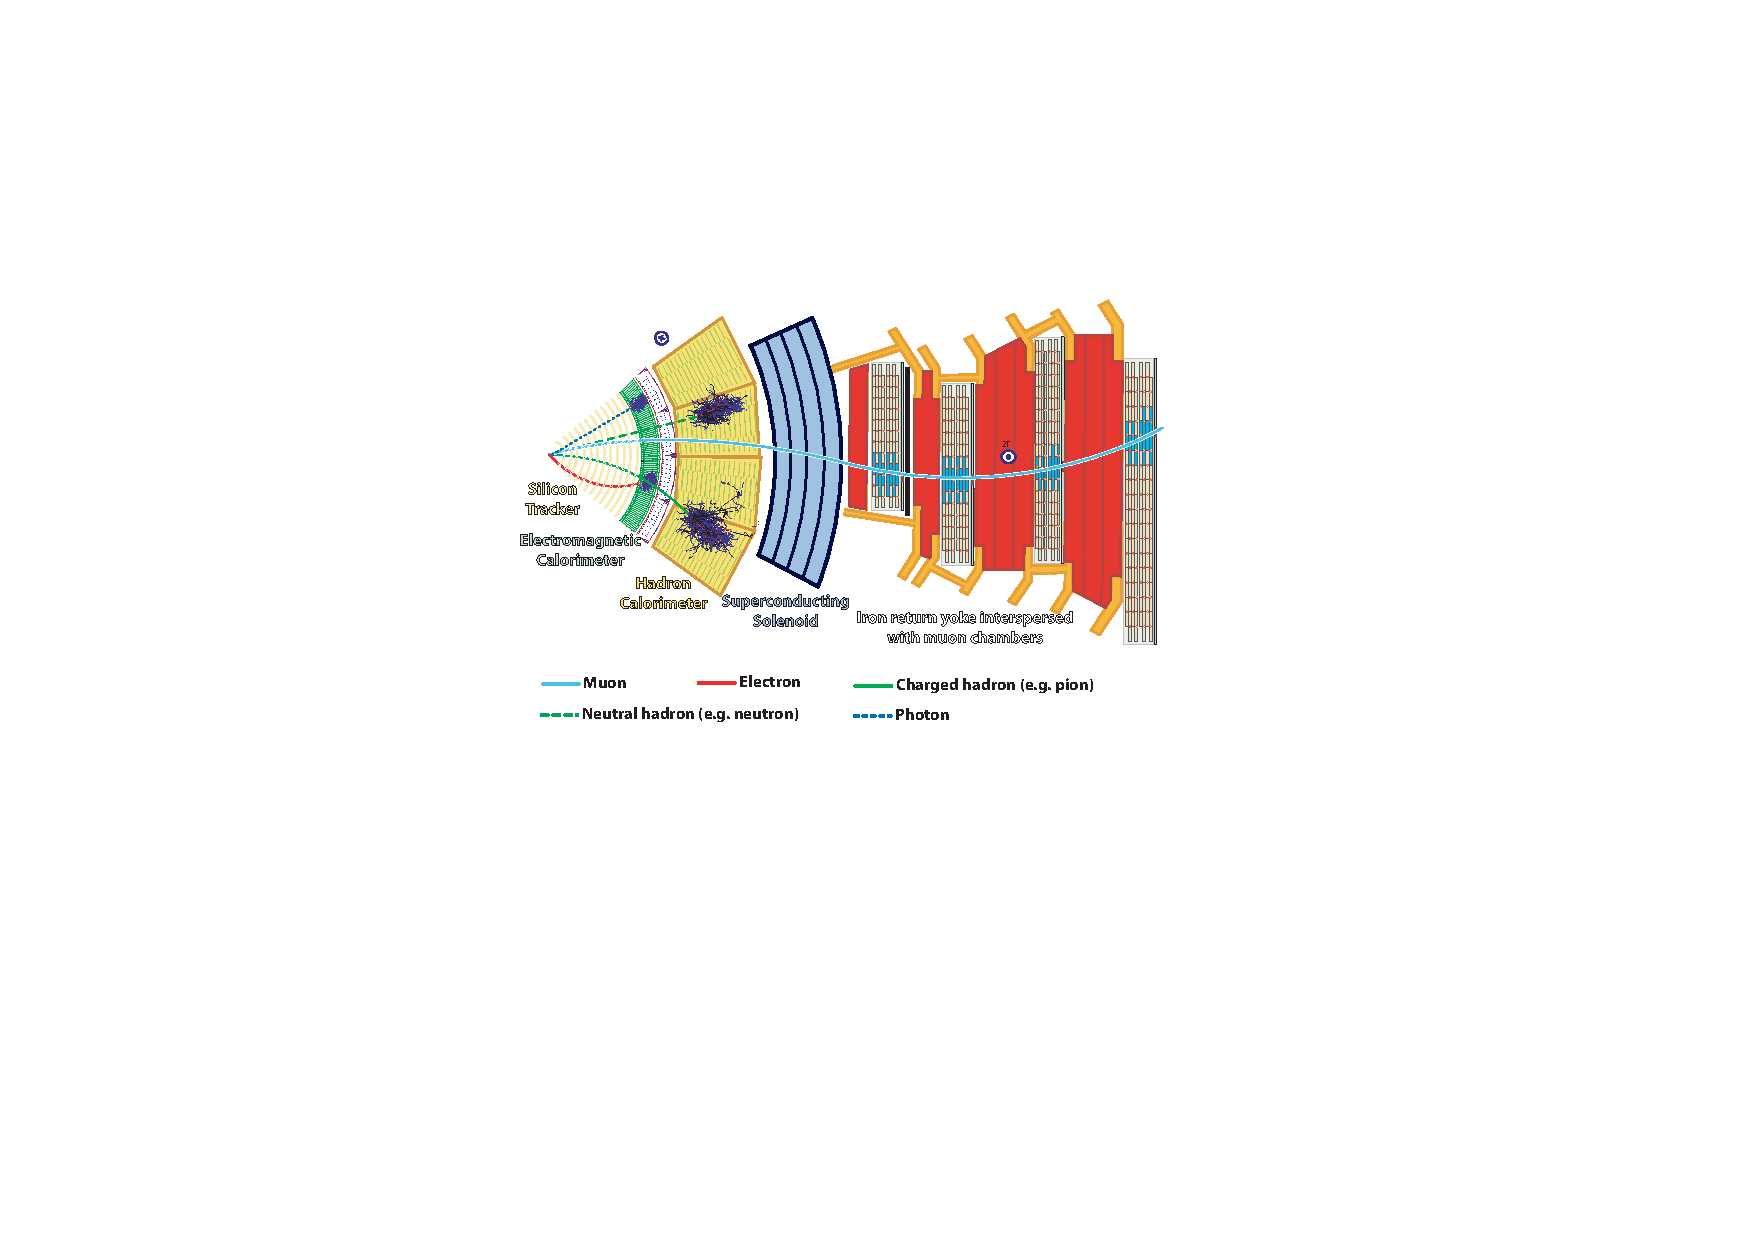
\includegraphics[width=0.5\textwidth]{slice}
  \caption{The path of different particles through a cross section of the CMS detector.}
  \label{reco:crosssec}
\end{figure}

\section{Electrons}
\todo[inline]{Why are electrons important phsyics objects}
\todo[inline]{Describe path that electrons make through the detector.}

\subsection{Triggering}

\subsection{Reconstruction}
Electrons are reconstructed in CMS using information from the pixel detector,
silicon strip tracker and the ECAL.

\subsubsection{Electron Clustering}
As electrons traverse the CMS tracker, the strong magnetic field causes the path
of the electrons to be curved in the azimuthal, $\phi$, direction. The electrons
radiate bremsstrahlung photons, so that when the electron energy reaches the
ECAL it is spread over a narrow strip in the phi direction.
\FigureRef{reco:brem} shows the fraction of energy radiated by bremsstrahlung for
electrons of energy $10$, $30$ and \unit{$50$}{\GeV}.

\begin{figure}[htb]
  \centering
  %\includegraphics[width=0.5\textwidth]{placeholder}
  \missingfigure{Fraction of energy radiated by bremsstrahlung from Electron
reconstruction in CMS}
  \caption{Fraction of electron energy, $E^{e}$, radiated away as bremsstrahlung
photons, $\sum E_{brem}^{\gamma}$ for electrons of energy }%$10$, $30$ and \unit{$50$}{\GeV}. From \cite{}.}
  \label{reco:brem}
\end{figure}

To measure the electron energy, including the bremsstrahlung photons, the
seperated deposits of energy need to be collected, using super-clustering
algorithms. 

In the barrel a ``hybrid'' algorithm is used. The hybrid algorithm proceeds by
identifying several hot crystals, with energies above a certain threshold, that
will act as seeds. The algorithm then forms $1\times3$ or $1\times5$ crystal
``dominos'', centered on the seed crystal, depending on the energy within the
domino. The dominos are then collected together in the $\phi$ direction, up to
an extension of \unit{0.3}{\rad}, to form clusters of clusters. This is
demonstrated in \FigureRef{fig:hybrid}.

\begin{figure}[htb]
  \centering
  %\includegraphics[width=0.5\textwidth]{placeholder}
  \missingfigure{hybrid clustering algorithm}
  \caption{Demonstration of the clustering of dominos in the hybrid algorithm.}
  \label{reco:hybrid}
\end{figure}

A ``multi5x5'' algorithm is used in the ECAL endcaps. Energy is collected in
$5\times5$ matrices, which are then collected together if their position lies on
a narrow $\phi$ road to form superclusters.

\subsubsection{Electron Seeding}
The superclusters are then used to select seeds for the track reconstruction.
Starting with a supercluster that passes a \pt and a hadronic veto, the
trajectory of the electron is propogated back through the magnetic field and
matched to the trajectory seeds, pairs or triplets of hits in the inner tracker.
If the trajectory seeds fall within a window of the supercluster path under
either charge hypothesis, they are selected and used to seed the track
reconstruction.
The ECAL driven seeding is comlemented by a tracker driven seeding algorithm.
This starts with high purity tracks and extrapolating them outwards to the ECAL.
This is effective for lower \pt electrons.

Seeds from both of the algorithms are collected and merged in to a single
collection, which is then used to seed the electron track reconstruction.

\subsubsection{Electron Track Reconstruction}
\todo[inline]{Rewrite this section}
The track reconstruction is based on a combinatorial Kalman filter,\todo{find a
citation for this} with the electron energy losses described using Bethe Heitler
modelling.

The track reconstruction starts with a seed, from which a tree of possible track
candidates is built from. 

%track reconstruction paper
Throughout the track reconstruction, tracks candidates are described by a state
vector containing information on the momentum, direction and position of the
track.

The Kalman filter is a
two step process. In the propogation step, track states are extrapolated to
the next layer of the detector, while taking in to account for energy losses due
to bremsstrahlung and coulomb scattering. 
In the update step, the extrapolated track state is 
combined with what is observed in that layer and the track is updated. 

The collected hits are passed to the GSF for a final fitting and estimation of
the track parameters. The GSF algorithm is similar to the Kalman filter but
energy losses are now described by a weighted sum of Gaussian distributions.
% corrections

\subsection{Electron Identification}
Electron identifiaction is based on a limited number of variables.
\todo{backgrounds to prompt electrons}

\subsubsection{Shape variable }

$\sigma_{\eta\eta}$ is the width of the electron shower in the $\eta direction$,
\begin{equation}
\sigma_{\eta\eta} = 
\sum_{\text{crystals}} \left(\eta_{i} - \eta{s}\right)^{2}
\frac{E_{i}}{E_{\text{seed cluster}}}.
\end{equation}

\subsubsection{Hadronic Energy}
Ratio of the energy deposited in the HCAL tower behind the electromagnetic seed
cluster to the energy of that seed cluster.

\subsubsection{Angular Separation of Track and Super Cluster}
$\Delta\phi$ and $\Delta\eta$ represent the angular separation between the
trajectory of the reconstucted GSF track, extrapolated to the ECAL, and the ECAL supercluster in the $\phi$
and $\eta$ direction respectivly.
\begin{align}
|\Delta\eta| &\equiv |\eta_{\text{SC}} - \eta_{track}|\\
|\Delta\phi| &\equiv |\phi_{\text{SC}} - \phi_{track}|
\end{align}

\subsubsection{Isolation}
For the calorimeter quantities

\subsubsection{Conversion Rejection}
Three further variables are included to reject electrons that are produced from
photon conversions. The missing hits is simply the number of layers in the inner
tracker where an expected hit from the track reconstruction is not detected by
the detector.
\todo{coversion partner tracks and dist and cot}
Coversion partner tracks are track candidates that are with in a cone of $\Delta
R < 0.3$ around the electron candidate track, and have an opposite charge. The
following two variables are used to detect \todo{what?} conversions.

\begin{equation}
\Delta \cot \theta \equiv \cot(\theta_{\text{KF}}) - \cot(\theta_{\text{GSF}})
\end{equation}
where $\theta_{KF}$ and $\theta_{GSF}$ are the polar angle of the conversion
partner track and the GSF track of the electron respectivly.

The variable, dist, is the distance between the two tracks where they are
parralel. \FigureRef{fig:dist} describes dist.

\begin{figure}[htb]
  \centering
  \missingfigure{Explanation of dist}
  %\includegraphics[width=0.5\textwidth]{placeholder}
  \caption{Dist is the distance between}
  \label{fig:dist}
\end{figure}

\subsubsection{Electron Identification Working Points}

Several sets of cuts have been produced for CMS analyses with different
efficiencies in mind. The cut values are sumarised in \TableRef{tab:electronwp}.
\todo{table of electron working points}

\subsection{Charge Identification}
The charge of an electron can be identified by studying how the electron trajectory
is bent in the magnetic field as the electron passes through the tracker. This
can be made difficult by conversion of bremsstrahlung photons when they are
radiated early. 

Within CMS, three methods of charge identifaction have been developed based on
the GSF track charge, the general track charge and the supercluster charge. The
GSF track charge is simply the sign of the curvature of the GSF fit of the
electron track. The general track charge is found by matching the GSF track with
general Kalman filter track by asking for shared hits in the pixel tracker. 
The super cluster charge is obtained by finding the sign of the phi difference
between the supercluster position and the first hit of the electron track.

At the \PZ peak, a charge mis-identification rate of \unit{3}{\%} is expected,
when using the electron trajectory from the GSF fit.  A sample with improved
charge identifaction can be obtained by using a majority method, that combines
the three measurements and assigns the sign from the 2 estimates out of three
that are in agreemenet, or by requiring that all three methods for assigning
charge are in agreement and discarding the event otherwise.

\section{Missing Energy}
\todo[inline]{Describe how MET is measured in CMS} 

\subsection{Particle Flow at CMS}
\todo[inline]{Tie particle flow in with rest of chapter.} 

New physics will manifest itself in CMS through signatures involving standard
model particles. Important signatures for many new phenomena include high \Pt\
jets, missing transverse energy (\met), jets containing \Pbottom quarks and
hadronically decaying tau leptons. To study these signatures it is important to
reconstruct and identify all particles in events as accurately as possible. The
particle-flow event reconstruction attempts to reconstruct and identify all
stable particles in an event by combining information from all CMS
sub-detectors. The particle reconstruction and identification starts with
collecting information from each subdetector to form elements such as tracks
and energy clusters in the calorimeters. These basic 'elements' are then
combined to form blocks which are then interpreted in terms of particles by the
particle flow algorithm. A list of individual particles is then returned from
the algorithm which can be used to study the event in greater detail by,
amongst other things, building jets, tagging b quarks and calculating missing
transverse energy.\cite{PF}

The first step of the particle-flow reconstruction algorithm is to collect the
fundamental elements. The elements consist of charged particles tracks from the
tracker, clusters of energy deposition in the calorimeters and muon tracks.
These elements need to be identified with a high efficiency and low fake rate
since the particle reconstruction depends on these basic elements and
misidentified elements could lead to missing or double counted
particles.\cite{PF}

As a particle traverses the detector it may interact with many CMS subdetectors
creating several particle-flow elements. A link algorithm is used to connect
the elements together to form blocks that typically contain 1, 2 or 3 elements.
The algorithm returns a distance between the elements as a measure of the
quality of the link. The final step of the particle flow algorithm is to
reconstruct and identify particles from each block of linked elements.\cite{PF}

Once the event has been fully reconstructed with the particle flow technique
the missing transverse energy (\met) in the event can be easily computed by
summing up the transverse momentum of all the reconstructed particles.\cite{PF}


  \chapter[Electron Charge Asymmetry]{ Measurement of the electron charge asymmetry with \unit{36}{\invpb} }

In this chapter the first measurement of the electron charge asymmetry in
inclusive \inclusiveWe production with the \ac{CMS} detector is described.
The analysis is performed on the full 2010 dataset, which corresponds to a
luminosity of \unit{36.1}{\invpb}.

\section{Event Selection}

The event selection is performed on a single electron dataset. This dataset is
formed of events that are selected using various single photon and single
electron triggers. From this dataset, electrons are selected that pass a limited
number of cuts. Events that contain only a single electron are then selected for
the analysis.

\subsection{Trigger}

\label{asym36:triggerdef}
Several triggers were used to select the events, due to the increasing
luminosity in the \ac{LHC} 2010 run.
In the initial runs, events were selected using only a single photon trigger. 
As the luminosity increased these triggers became prescaled, it was
necessary to use electron triggers to select events. 
As the luminosity increased even further, it was necesary to use electron
triggers that included cuts on certain electron ID variables.

The triggers used to select the events are sumarised in \TableRef{asym36:triggers}
where ``HLT\_Ele$X$'' indicates a selection requiring an electron with  $\Pt > \unit{X}{\GeV}$. 
``Photon'' in the name indicates that the selection was applied to ECAL
superclusters rather than a reconstructed electron. 
``SW'' stands for small window, where window refers to the electron
pixel-matching window. 
 ``Cleaned'' indicates that spikes in the \ac{ECAL} have been removed.  \todo{define spikes?}

``CaloEleId'' and ``TightCaloIdIso'' represent increasingly tighter selection
based on the shower shape ID and isolation variables from only the \ac{ECAL},
and not the $\Delta\phi$ or $\Delta\eta$ variables.  

``TightCaloIdIso'' indicates a tight selection based on all ID variables. 
This nullifies the inverted cuts used for the control region but
it was the only trigger available for these runs without a prescale applied.
To compensate for the missing events in the control region, a looser prescaled
trigger was also applied in these runs.

\begin{table}[htbp]
  \centering
  \begin{tabular}{ l l }
    \toprule
    Run Ranges & Trigger String\\
    \midrule
    132440-137028 & \verb=HLT_Photon10_L1R= \\
    138564-140401 & \verb=HLT_Photon15_Cleaned_L1R= \\
    141956-144114 & \verb=HLT_Ele15_SW_CaloEleId_L1R= \\
    146428-147116 & \verb=HLT_Ele17_SW_CaloEleId_L1R= \\
    147196-148102 & \verb=HLT_Ele17_SW_TightEleId_L1R= \\
                  & \verb=HLT_Ele17_SW_L1R (prescaled)= \\ 
    148822-149063 & \verb=HLT_Ele22_SW_TighterCaloIdIso1_L1R_v1= \\
    149181-149442 & \verb=HLT_Ele22_SW_TighterCaloIdIso1_L1R_v2= \\
    \bottomrule
  \end{tabular}
  \caption{Triggers used to select the data used in this analysis.}
  \label{asym36:triggers}
\end{table}

\subsection{Event Selection}
An Event is selected if it contains a single electron that passes all the electron
selection requirements.
To remove Drell-Yan events, an event is vetoed if it contains a second lepton
(an electron passing a loose selecton, or an isolated muon) with $\PT > 
\unit{15}{\GeV}$.

The exected composition of the selected events, derived from MC simulation
samples, is shown in \TableRef{asym36:selectedcomp}. With a \pT cut of
\unit{25}{\GeV} it is expected that the selected events are \unit{$\approx
65$}{\GeV} signal events, and of the remaing \unit{35}{\%} background events, the
majority of them are \ac{QCD} background events with a small ammount of \ac{EWK}
events. 

\begin{figure}[htbp]
  \begin{center}
    \includegraphics*[width=0.85\textwidth]{pfmet_dist}
    \caption{Particle Flow transverse missing energy (PFMET) distribution for selected events.}
  \label{fig:pfmet}
  \end{center}
\end{figure}

The Particle Flow \ETm distribution for the events that pass the event
selection, with an electron cut of $\PT > \unit{25}{\GeV}$ and $|\eta| < 2.4$ is
shown in \FigureRef{fig:pfmet}. There are two obvious peaks in the
distribution. The peak at \unit{$\ETm \approx 40$}{\GeV} is the
\HepProcess{\PW\to\Pelectron\Pnue} signal region. This region will also contain
\HepProcess{\PW\to\Ptau\Pnut} backgrounds. The peak at
\unit{$\ETm\approx 10$}{\GeV} is the background region that contains the \ac{QCD}
and \ac{DY} background events.

\begin{table}[htbp]
\begin{center}
%\begin{sideways}
\begin{tabular}{lcrrr}
    \toprule
  $|\eta|$ range & Charge & \multicolumn{3}{c}{Selected Events}\\
                 &        & $\PT>25$ \GeV & $\PT>30$ \GeV & $\PT>35$ \GeV\\
\midrule
$0.0<| \eta |<0.4$ &+& 18956&14232&9885\\
                   &-& 15060&11505&8105\\
$0.4<| \eta |<0.8$ &+& 20118&14966&10345\\
                   &-& 15736&11780&8307\\
$0.8<| \eta |<1.2$ &+& 20681&15091&10184\\
                   &-& 16167&11735&8112\\
$1.2<| \eta |<1.4$ &+& 10646&7606&5161\\
                   &-& 8226&5871&4067\\
$1.6<| \eta |<2.0$ &+& 16426&11877&7814\\
                   &-& 11678&8578&5886\\
$2.0<| \eta |<2.4$ &+& 18885&13239&8726\\
                   &-& 13226&9227&6184\\
    \bottomrule
\end{tabular}
%\end{sideways}
\end{center}
\caption{Number of events passing the event selection for lepton momentum cut of $\PT>25$ \GeV, $\PT>30$ \GeV and $\PT>35$ \GeV .}
    \label{asym36:selectedevents}
\end{table}

The number of selected events that pass the
event selection are shown in \TableRef{asym36:selectedevents}. To obtain a
measurement of the asymmetry from the selected events it is necesary to extract
the signal yield from each pseudorapidity/charge bin.

\begin{table}[htbp]
\begin{center}
\begin{tabular}{llrrr}
    \toprule
& & $\PT>25$ \GeV & $\PT>30$ \GeV & $\PT>35$ \GeV  \\
\midrule
Signal & \HepProcess{\PW\to\Pe\Pnu} & $65.1\%$&$63.5\%$ &$60.2\%$ \\
EWK & \HepProcess{\PZ\to\Ptau\Ptau} & $0.4\%$ &$0.3\%$  &$0.2\%$ \\
    & \HepProcess{\PZ\to\Pe\Pe}     & $4.1\%$ &$3.5\%$  &$3.0\%$\\
    & \HepProcess{\PW\to\Ptau\Pnu}  & $1.9\%$ &$1.1\%$  &$0.6\%$\\
    & \HepProcess{\Ptop\APtop}      & $0.3\%$ &$0.3\%$  &$0.3\%$\\
    & Total                         & $6.7\%$ &$5.2\%$  &$4.1\%$\\
QCD & Total                         & $28.2\%$&$31.3\%$ &$35.7\%$\\
    \bottomrule
\end{tabular}
\caption{Composition of selected events for lepton momentum cut of $\PT>25$ \GeV, $\PT>30$ \GeV and $\PT>35$ \GeV .}
\label{asym36:selectedcomp}
\end{center}
\end{table}

The exected composition of the selected events, derived from MC simulation
samples, is shown in \TableRef{asym36:selectedcomp}. With a \pT cut of
\unit{25}{\GeV} it is expected that the selected events are \unit{$\approx
65$}{\GeV} signal events, and of the remaing \unit{35}{\%} background events, the
majority of them are \ac{QCD} background events with a small ammount of \ac{EWK}
events. 

\subsection{Fit Results}
The results of the extended maximum liklihood fits to each pseudorapidity/charge
bin are shown in \FigureRef{fig:fit1} and \FigureRef{fig:fit2}.
The ratio between the fits and the data for each of the 
bins are shown in \FigureRef{fig:fit1ratio} and \FigureRef{fig:fit2ratio}.
The signal yield in each bin is summarised in \TableRef{tab:rawasym} and the
$\chi^2$ of each fit is noted in \TableRef{tab:chi2}.

\begin{table}[htbp]
\begin{center}
%\begin{sideways}
\begin{tabular}{lcrrr}
    \toprule
$|\eta|$ range & Charge & \multicolumn{3}{c}{Signal Yield}\\
               &        & $\PT>25$ \GeV & $\PT>30$ \GeV & $\PT>35$ \GeV  \\
\midrule
$0.0<| \eta |<0.4$ &+&-&-&-\\
                   &-&-&-&-\\
$0.4<| \eta |<0.8$ &+&-&-&-\\
                   &-&-&-&-\\
$0.8<| \eta |<1.2$ &+&-&-&-\\
                   &-&-&-&-\\
$1.2<| \eta |<1.4$ &+&-&-&-\\
                   &-&-&-&-\\
$1.6<| \eta |<2.0$ &+&-&-&-\\
                   &-&-&-&-\\
$2.0<| \eta |<2.4$ &+&-&-&-\\
                   &-&-&-&-\\
    \bottomrule
\end{tabular}
%\end{sideways}
\end{center}
\caption{Signal yield}
    \label{fig:sigyield}
\end{table}

\begin{table}[htbp]
\begin{center}
\begin{tabular}{lcr}
    \toprule
$|\eta|$ range &Charge & $\chi^2$/ndof of Fit\\
\midrule
$0.0<| \eta |<0.4$ &+&  0.86\\
                   &-&  0.84\\
$0.4<| \eta |<0.8$ &+&  0.99\\
                   &-&  1.36\\
$0.8<| \eta |<1.2$ &+&  1.05\\
                   &-&  1.13\\
$1.2<| \eta |<1.4$ &+&  0.97\\
                   &-&  1.30\\
$1.6<| \eta |<2.0$ &+&  1.38\\
                   &-&  1.61\\
$2.0<| \eta |<2.4$ &+&  1.44\\
                   &-&  1.11\\
    \bottomrule
\end{tabular}
\caption{\label{tab:chi2}$\chi^2$/ndof of Fit.}
\end{center}
\end{table}

\section{Systematic Uncertainties}
The following section will describe the main sources of systematic uncertainty
for this measurement. 

\subsection{Relative Efficiency}

If the reconstruction efficiency of electrons is different to that of positrons
then the measured asymmetry wil be diluted and will need to be corrected for
the relative efficiency.

\begin{equation}
A_{exp}(\eta) = \frac{
                    \frac{dN}{d\eta}(e^+)-
                    \frac{\epsilon^+}{\epsilon^-}\frac{dN}{d\eta}(e^-)
                }
                {
                    \frac{dN}{d\eta}(e^+)+
                    \frac{\epsilon^+}{\epsilon^-}\frac{dN}{d\eta}(e^-)
                }
\end{equation}

The efficiency for electrons and positrons is measured using the tag and probe
method \todo{reference the CMS tag and probe method paper/note}
with a sample of \Zee events from the same datasets used in the analysis. 
The \Zee events offer a high purity source of unbiased electrons with which to
measure the efficiencies.

From the sample of \Zee events a ``tag'' electron is selected with a strict
selection criteria. 
A ``probe'' electron is selected with the same electron selection decribed
earlier.
The invariant mass of the tag-probe pair is required to be
$\unit{60}{\GeV} < M_ee < \unit{120}{\GeV}$ to ensure a high purity sample.

Efficiencies can then be calculated by measuring the signal yield in events
with one tag electron and one probe passing the selection (tag \& pass) and
events where the probe electron fails the selection (tag \& fail).
The signal yield is extracted using an simultaneous maximum likelihood fit to
both the tag \& pass and the tag \& fail samples.

For this analysis the efficiencies are measured in two parts:

\begin{itemize}
    \item GSF tracking efficiency
    \item Identification efficiency, including conversion rejection, unaminous
charge assignment and HLT request.
\end{itemize}

\begin{table}[htbp]
\begin{center}
\begin{sideways}
\begin{tabular}{cccccccc}
    \toprule
$|\eta|$  & \multicolumn{3}{c}{GSF tracking } & \multicolumn{3}{c}{ID } & $R_\epsilon$ \\
region    & $\epsilon_{GSF}^+$ (\%) &$\epsilon_{GSF}^-$ (\%) & $R_{\epsilon_{GSF}}$ 
                                              & $\epsilon_{ID}^+$ (\%) &$\epsilon_{ID}^-$ (\%) & $R_{\epsilon_{ID}}$ &  \\
\midrule
$\left[ 0.0,0.4 \right]$ & 95.7$\pm$1.1 & 97.5$\pm$1.0 & 0.982$\pm$0.015 & 71.2$\pm$1.5 & 68.4$\pm$1.5 & 1.04$\pm$0.03 &1.02$\pm$0.035  \\
$\left[ 0.4,0.8 \right]$ & 98.8$\pm$ 1.0& 98.5$\pm$1.1 & 1.003$\pm$0.015 & 72.5$\pm$1.7 & 75.6$\pm$1.6 & 0.96$\pm$0.04 &0.96$\pm$ 0.04 \\
$\left[ 0.8,1.2 \right]$ & 97.6$\pm$ 1.0& 98.4$\pm$1.0 & 0.992$\pm$0.015 & 77.4$\pm$1.5 & 74.4$\pm$1.7 & 1.04$\pm$0.04 &1.03$\pm$ 0.04 \\
$\left[ 1.2,1.4 \right]$ & 96.2$\pm$ 1.5& 96.3$\pm$1.5 & 0.999$\pm$0.022 & 69.3$\pm$2.7 & 73.0$\pm$2.6 & 0.95$\pm$0.05 &0.95$\pm$0.05  \\
$\left[ 1.6,2.0 \right]$ & 96.8$\pm$ 1.2& 96.9$\pm$1.0 & 0.999$\pm$0.015 & 61.9$\pm$2.0 & 63.6$\pm$2.0 & 0.97$\pm$0.05 &0.97$\pm$0.05  \\
$\left[ 2.0,2.4 \right]$ & 96.4$\pm$ 1.1& 97.0$\pm$1.0 & 0.994$\pm$0.015 & 58.2$\pm$2.1 & 56.7$\pm$2.1 & 1.03$\pm$0.05 &1.02$\pm$0.05  \\
\midrule
$\left[ 0.0,1.4 \right]$ & 98.8$\pm$0.5 & 98.4 $\pm$0.5 & 1.004$\pm$0.007 & 84.1$\pm$0.8 & 83.8$\pm$0.8 & 1.003$\pm$0.014 & 1.007$\pm$ 0.015 \\
$\left[ 1.6,2.4 \right]$ & 98.3$\pm$0.7 & 97.8 $\pm$0.7 & 1.005$\pm$0.010 & 70.7$\pm$1.4 & 71.5$\pm$1.4 & 0.99$\pm$0.03 &0.99$\pm$ 0.03 \\
\midrule 
$\left[ 0.0,2.4 \right]$ & 98.5$\pm$0.4 & 97.8$\pm$0.4 & 1.007$\pm$0.006 & 80.3$\pm$0.7 & 80.3$\pm$0.7 & 1.000$\pm$0.012 &1.007$\pm$0.014  \\
    \bottomrule
\end{tabular}
\end{sideways}
\end{center}
\caption{ GSF tracking and identification efficiency as a function of charge.}
\label{asym36:tagprobe}
\end{table}

The \TableRef{asym36:tagprobe} shows the GSF tracking effiency and identifcation 
effiency as a function of the charge.

The relative efficiency: 

\begin{equation}
R_\epsilon  =  \frac{\epsilon^+}{\epsilon^-}
\end{equation}

is found to be statistically compatible with 1 so the measured asymmetry is not
corrected for this effect.

The main systematic errors on the efficiency measurements are the energy scale
and the signal shape used to extract the signal yield. Fortunately, these
errors will cancel in the calculation of the ratio $R_\epsilon$, the difference
on  $R_\epsilon$ introduced by the energy scale and signal shape is negligable
when compared to the statistical uncertainty of the measurement, so only the
statistical uncertainty is propogated to the error in the ratio,
$dR_\epsilon$.

\begin{equation}
  \label{eq:releff}
  \sigma_{\mathcal{A}} =\mathcal{}(R_\epsilon=1) - \mathcal{A}(R_\epsilon=1\pm dR_\epsilon)  \simeq \frac{dR_\epsilon}{2}(1-\mathcal{A}^2)\simeq \frac{dR_\epsilon}{2}
\end{equation}


\subsection{Signal Extraction Method}

The systematic uncertainty due to the siganl extraction method is evaluated be
considering the error introduced be each \ETm tempalte shape used in the fit
separately.

\subsubsection{Background \ETm Shape}

The \ac{QCD} and \gjet \ETm template shape is obtained from a control sample of
events by antiselecting electrons. This may introduce a systematic bias to the
measurement if there is a difference between the anti-selected \ac{QCD} and \gjet
\ETm samples and the selected \ac{QCD} and \gjet samples.

The systematic uncertainty due to the \ac{QCD} and \gjet \ETm shape is evaluated by
varying the anti-selection used to obtain the control sample and observing the
effect that this has on the measured asymmetry.

For each variation on the antiselection, 500 pseudo-data experiments are
generated with the number of events that are expected in \unit{36.1}{\invpb} of
data. The distribution of the measured asymmetry is then fitted with a
gaussian.
The effect that changing the anti-selection has on the mean of the guassian is
studied, the maximum distance from the asymmetry measured with the nominal
anti-selection is taken as an estimate of the systematic uncertainty.

\begin{table}[htbp]
\begin{center}
\begin{tabular}{crr}
    \toprule
$|\eta|$  &\multicolumn{2}{c}{ $\sigma(\mathcal{A}) \times 10^{-4}$}\\
   range      & MC & Data\\
\midrule
$0.0<|\eta|<0.4$ & 8 & 12\\
$0.4<|\eta|<0.8$ & 7 & 9\\
$0.8<|\eta|<1.2$ & 8 & 21\\
$1.2<|\eta|<1.4$ & 12& 25\\
$1.6<|\eta|<2.0$ & 6 & 10\\
$2.0<|\eta|<2.4$ & 22& 13\\
    \bottomrule
\end{tabular}
\caption{Maximum distance between the asymmetry measured with many different antiselections
and the asymmetry measured with the chosen antiselection in MC pseudo data and real data for each eta bin.}
\label{tab:systQCD}
\end{center}
\end{table}


\subsubsection{Signal \ETm Shape from Boson Recoil}

The signam \ETm shape is constructed using information from the boson recoil.
There are three main sources of uncertainty due to the signal template,

\begin{itemize}
    \item the uncertainty in the recoil corrections,
    \item the effect the energy scale has on the recoil corrections,
    \item the uncertainty on the \ac{PDF} used to generate the events that the
recoil corrections are applied to.
\end{itemize}

To evaluate the effect of the uncertainties of the recoil method, the upper and
lower limits on the corrections are used to generate different tempaltes, and
the effect on the measured asymmetry is evaluated as a measure of the
systematic uncertainty.

The recoil method uses generator level \ac{MC} simulation as an input to the
template shape. To evaluate the efect of the generator used, templates are
generated with the CTEQ 6.6 \todo{cite the CTEQ guys here}
uncertainty \acp{PDF} which contain the central \ac{PDF} and 44 error \acp{PDF}
which contain the \unit{95}{\%} \ac{CL} for each of the 22 free parameters in
the \ac{PDF}. The maximum change in distance with respect to the central value
is taken as a measure of the systematic uncertainty.

Any differences in the energy scale of the electrons between data and \ac{MC}
must be taken in to account to ensure accurate \ETm predictions. The \ac{MC} energy
scale corrections were determined from \PZ data and applied to the \PZ \ac{MC}
before calculating the recoil components \cite{recoil}.

\begin{table}[htbp]
\begin{center}
\begin{tabular}{crrrr}
    \toprule
$|\eta|$   & \multicolumn{4}{c}{$\sigma(\mathcal{A}) \times 10^{-4}$}\\
range      & Recoil Corr. & Energy Scale & PDF & Combined \\
\midrule
$0.0<|\eta|<0.4$ &  4 & 2 & 10  & 11 \\
$0.4<|\eta|<0.8$ &  6 & 3 & 15  & 16 \\
$0.8<|\eta|<1.2$ &  5 & 2 & 15  & 16 \\
$1.2<|\eta|<1.4$ &  9 & 5 & 20  & 22 \\
$1.6<|\eta|<2.0$ & 11 & 4 & 20  & 23 \\
$2.0<|\eta|<2.4$ &  7 & 3 & 20  & 21 \\
    \bottomrule
\end{tabular}
\caption{\label{tab:systSIG}Systematic uncertainty due to the Signal \ETm shape used in the signal
extraction method assigned to each eta bin.}
\end{center}
\end{table}

\subsubsection{\ac{EWK} \ETm Shape}

The \ac{EWK} shape is also generated from \ac{MC} samples. During the fitting
procedure, the \ac{EWK} shape is fixed to the \Wenu signal shape according to
the cross section taken from the \ac{MC} samples. To estimate the effect of the
uncertainty of the cross section has on the asymmetry measurement, the \ac{EWK}
background is artificially varied by \unit{$\pm20$}{ \% } and the effect on the
asymmetry is measured. Even with an over estimation of the uncertainty on the
cross section, the effect on the asymmetry is found to be small.

\begin{table}[htbp]
\begin{center}
\begin{tabular}{cr}
    \toprule
$|\eta|$ range & $\sigma(\mathcal{A}) \times 10^{-4}$\\
\midrule
$0.0<|\eta|<0.4$ & 0\\
$0.4<|\eta|<0.8$ & 3\\
$0.8<|\eta|<1.2$ & 1\\
$1.2<|\eta|<1.4$ & 1\\
$1.6<|\eta|<2.0$ & 0\\
$2.0<|\eta|<2.4$ & 3\\
    \bottomrule
\end{tabular}
\caption{\label{tab:systEWK}Systematic uncertainty due to the electroweak \ETm shape used in the signal extraction method assigned to each eta bin.}
\end{center}
\end{table}


\subsection{Charge Misassignment}

The charge misassignment rate, $\omega$, is the rate at which electrons are
misasigned as positive charge and identified as positrons, and vice versa. The
misassignment induces a dilution factor to the asymmetry as a function of the
electron pseudorapidity. If it is assumed that the misassignment rate of
electrons to positrons is the same as the rate of positrons to electrons, \ie 

\begin{equation}
  \omega( \HepProcess{\APelectron \to \Pelectron} ) =
  \omega( \HepProcess{\Pelectron \to \APelectron} )
\end{equation}

then the dilution factor is given by $(1-2\omega_\eta)$ and the measured
asymmetry must be corrected by the following relation

\begin{equation}
  A_{exp}(\eta) = (1-2\omega_\eta)
                \frac{
                    \frac{dN}{d\eta}(e^+)-
                    \frac{\epsilon^+}{\epsilon^-}\frac{dN}{d\eta}(e^-)
                }
                {
                    \frac{dN}{d\eta}(e^+)+
                    \frac{\epsilon^+}{\epsilon^-}\frac{dN}{d\eta}(e^-)
                }
\end{equation}

The rate of charge misassignment is obtained from \Zee samples selected with
the same selection used in the analysis. The rate is measured by comparing the
same sign \PZ\ yield (\HepProcess{\PZ\to\Pepm\Pepm}) to the opposite sign \PZ\
yield (\HepProcess{\PZ\to\Pepm\Pemp}).

\begin{table}[htbp]
  \begin{center}
\begin{tabular}{lrrrr}
\toprule
$\eta$ range        & $\omega \times 10^{-4}$  & \multicolumn{3}{c}{$\sigma(\mathcal{A})_{misch}\times 10^{-4}$}\\
& & \PT $>$ 25 \GeV & \PT $>$ 30 \GeV & \PT $>$ 35 \GeV \\
\midrule
$0.0<| \eta |<0.4$  & $0^{+8}$          &  2 &  2 & 2 \\ 
$0.4<| \eta |<0.8$  & $8^{+8}_{-8}$     &  3 &  2 & 2 \\
$0.8<| \eta |<1.2$  & $11^{+10}_{-8}$   &  3 &  3 & 3 \\
$1.2<| \eta |<1.4$  & $34^{+21}_{-15}$  &  8 &  7 & 6 \\
$1.6<| \eta |<2.0$  & $41^{+20}_{-15}$  &  9 &  8 & 7 \\
$2.0<| \eta |<2.4$  & $25^{+21}_{-15}$  & 10 & 10 & 9 \\
\bottomrule
\end{tabular}
\caption{\label{tab:mischarge}Charge mismeasurement rate and systematic effect on the charge asymmetry.}
\end{center}
\end{table}

\subsection{Lepton Energy Scale and Resolution}

The energy resolution and scale of the electrons can introduce a systematic
error on the asymmetry due to the effect of of the transverse momentum cut
applied to the electrons. The largest source of electron scale bias is the
radiation induced change to the ECAL crystal transparency.

To correct fot this effect, energy scale and resolution corrrections are
derrived using a \Zee mass distribution. The corrections are parameterised by
six energy scale factors, $s_i$, and six resolutions, $\sigma_i$, one for each
pseudorapidity bin in the asymmetry measurement.
The scale factors represent the average factor each electrons \Pt in data
should be corrected to match the expected \ac{MC} energy scale.
The resolution factors represent the difference of the resolution in data and
\ac{MC}. It is the additional smearing that would need to be applied to
reconstruction level \ac{MC} to match the observed resolution in data.

A sample of \Zee events is  split in to 21 categories which correspond to all
combinations of pseudorapidity bins of the two electrons ($6+\binom{6}{2} = 21$).

A mass template s obtained in each category from \ac{MC} simulation where a
perfect \ac{ECAL} calibration is considered.

A simultaneous fit to the \Zee mass is performed in each of the 21 categories
to determine the six energy scale factors, $s_i$, and the six resolutions, 
$\sigma_i$.

In each category ($category_{ij}$) where one electron is in the $i^{th}$
pseudorapidity bin and the other is in the $j^{th}$ bin, the \ac{MC} template
mass shape is scaled by 

\begin{equation}
    \frac{1}{\sqrt{s_i s_j} } 
\end{equation}

and smeared by an addtional gaussian with width of 

\begin{equation}
    \sqrt{\sigma_i^2+\sigma_j^2}
\end{equation}

%TODO figures
\todo[inline]{Add figures to demonstrate this}

The corrections are applied to the electron before the final \Pt cut so tjat
the measured asymmetry is corrected for the energy scale.

A conservative uncertainty of \unit{1}{\% } is assigned to the electron energy
after the scale corrections. A systematic error is then estimated by measuring
the difference of the measured charge asymmetry with and without the additional
\unit{1}{\% } scale factor.

\begin{table}[htbp]
  \begin{center}
    \begin{tabular}{cccc}
    \toprule
$\eta$ range& $\sigma{\mathcal{A}} \times 10^{-4}$  & Additional $\sigma{E_{e^\pm}}$  & $\sigma{\mathcal{A}} \times 10^{-4}$ \\
& Perfect ECAL  & from fit  &  Realistic ECAL\\
& Calibration & (GeV) & Calibration \\
\midrule
$0.0<| \eta |<0.4$  &  8  & 0.2  &  4 \\
$0.4<| \eta |<0.8$  &  7  & 0.4  &  5\\
$0.8<| \eta |<1.2$  & 17  & 0.3  & 19\\
$1.2<| \eta |<1.4$  & 41  & 1.0  & 43\\
$1.6<| \eta |<2.0$  & 31  & 0.9  & 32 \\
$2.0<| \eta |<2.4$  & 41  & 0.3  & 42\\
    \bottomrule
    \end{tabular}
    \caption{\label{tab:acc}Systematic error for detector effects in the acceptace corrections.}
  \end{center}
\end{table}

\begin{table}[htbp]
  \begin{center}
    \begin{tabular}{cccc}
    \toprule
$\eta$ range& \PT $>$ 25 \GeV & \PT $>$ 30 \GeV & \PT $>$ 35 \GeV \\
\midrule
$0.0<| \eta |<0.4$  & 4 & 5 &-3 \\
$0.4<| \eta |<0.8$  & 5 & 9 & -10\\
$0.8<| \eta |<1.2$  & 19 & 9 & 32\\
$1.2<| \eta |<1.4$  & 43 &37 & 24\\
$1.6<| \eta |<2.0$  & 32 &50 & 43\\
$2.0<| \eta |<2.4$  & 42 &52 & 27\\
    \bottomrule
\end{tabular}
\caption{\label{tab:bias}Bias values due to the electron resolution for different lepton \PT cuts.}
  \end{center}
\end{table}

\begin{table}[htbp]
  \begin{center}
    \begin{tabular}{cccc}
    \toprule
$\eta$ range& \PT $>$ 25 \GeV & \PT $>$ 30 \GeV & \PT $>$ 35 \GeV \\
\midrule
$0.0<| \eta |<0.4$  & 10 & 5 & 14\\
$0.4<| \eta |<0.8$  & 7 & 15 & 44\\
$0.8<| \eta |<1.2$  & 2 & 24 & 31\\
$1.2<| \eta |<1.4$  & 19 & 27 & 46\\
$1.6<| \eta |<2.0$  & 24 & 17 & 28\\
$2.0<| \eta |<2.4$  & 16 & 17  & 44\\
    \bottomrule
\end{tabular}
\caption{\label{tab:AddScale}Systematic error due to the additional scale factor of 1\% on the energy.}
  \end{center}
\end{table}


\subsection{Systematic Uncertainty Summary}

\begin{table}[htbp]
\begin{center}
\begin{tabular}{ccccccc}
    \toprule
\multicolumn{7}{c}{$\sigma(\mathcal{A}) \times 10^{-4}$}\\
 & Relative   & Electron  & Signal     & Charge & \ETm & Total \\
 & Efficiency & Scale/Res & Estimation & MisID  & Scale/Res & \\
\midrule 
\multicolumn{7}{c}{$\PT > 25$ \GeV}\\
$0.0<|\eta|<0.4$ & 70 & 11 & 16 &  2 &  0 &  73\\
$0.4<|\eta|<0.8$ & 70 &  9 & 19 &  3 &  0 &  73\\
$0.8<|\eta|<1.2$ & 70 & 19 & 26 &  3 &  0 &  77\\
$1.2<|\eta|<1.4$ & 70 & 47 & 33 &  8 &  0 &  90 \\
$1.6<|\eta|<2.0$ & 70 & 40 & 25 &  9 &  0 &  85\\
$2.0<|\eta|<2.4$ & 70 & 45 & 25 & 10 &  0 &  87\\
\midrule
\multicolumn{7}{c}{$\PT > 30$ \GeV}\\
$0.0<|\eta|<0.4$ & 70 &  7 & 16 &  2 &  0 &  72 \\
$0.4<|\eta|<0.8$ & 70 & 17 & 19 &  2 &  0 &  75 \\
$0.8<|\eta|<1.2$ & 70 & 26 & 26 &  3 &  0 &  79 \\
$1.2<|\eta|<1.4$ & 70 & 46 & 33 &  7 &  0 &  91 \\
$1.6<|\eta|<2.0$ & 70 & 53 & 25 &  8 &  0 &  92 \\
$2.0<|\eta|<2.4$ & 70 & 55 & 25 & 10 &  0 &  93 \\
\midrule 
\multicolumn{7}{c}{$\PT > 35$ \GeV}\\
$0.0<|\eta|<0.4$ & 70 & 14 & 16 &  2 &  0 & 73 \\
$0.4<|\eta|<0.8$ & 70 & 45 & 19 &  2 &  0 & 85 \\
$0.8<|\eta|<1.2$ & 70 & 44 & 26 &  3 &  0 & 87 \\
$1.2<|\eta|<1.4$ & 70 & 52 & 33 &  6 &  0 & 93 \\
$1.6<|\eta|<2.0$ & 70 & 51 & 25 &  7 &  0 & 94 \\
$2.0<|\eta|<2.4$ & 70 & 52 & 25 &  9 &  0 & 94 \\
\bottomrule
\end{tabular}
\caption{\label{tab:summarysyst}Summary of the systematic errors}
\end{center}
\end{table}

\section{Results}
The measurement of the electron charge assymetry is presented with three
different \pT cuts of 25, 30 and \unit{35}{\GeV}. 

The results of the electron charge asymmetry with a \pT cut of \unit{25}{\GeV}
are summarised in \TableRef{tab:results25} and shown in
\FigureRef{fig:results25}.

\begin{figure}[htbp]
  \begin{center}
  \includegraphics*[width=0.45\textwidth,angle=90]{Asym_25}
  \caption{\label{fig:asym25} Measured electron charge asymmetry corrected with predictions from CTEQ10W and MSTW08NNLO.}
  \end{center}
\end{figure}

\begin{table}[htbp]
\begin{center}
\begin{tabular}{crrrr}
    \toprule
$|\eta|$ range & $<|\eta|>$ & Data & CTEQ6.6 & MSTW \\
\midrule 
$0.0<|\eta|<0.4$ & 0.2 & $0.1541\pm0.0064\pm0.0073$ & $0.1502^{+0.0062}_{-0.0045}$ & $0.1296^{+0.0022}_{-0.0032}$\\
$0.4<|\eta|<0.8$ & 0.6 & $0.1666\pm0.0064\pm0.0073$ & $0.1682^{+0.0060}_{-0.0055}$ & $0.1458^{+0.0023}_{-0.0031}$\\
$0.8<|\eta|<1.2$ & 1.0 & $0.1728\pm0.0065\pm0.0077$ & $0.1944^{+0.0051}_{-0.0072}$ & $0.1737^{+0.0026}_{-0.0030}$\\
$1.2<|\eta|<1.4$ & 1.3 & $0.1895\pm0.0096\pm0.0090$ & $0.2216^{+0.0050}_{-0.0087}$ & $0.1976^{+0.0032}_{-0.0026}$\\
$1.6<|\eta|<2.0$ & 1.8 & $0.2331\pm0.0076\pm0.0085$ & $0.2672^{+0.0047}_{-0.0105}$ & $0.2454^{+0.0039}_{-0.0018}$\\
$2.0<|\eta|<2.4$ & 2.2 & $0.2670\pm0.0077\pm0.0087$ & $0.2821^{+0.0037}_{-0.0110}$ & $0.2619^{+0.0039}_{-0.0018}$\\
    \bottomrule
\end{tabular}
\caption{Measured electron charge asymmetry with predictions from CTEQ6.6 and MSTW PDFs.  36 Uncertainties on measured asymmetry are statistical and systematic respectivly and the Uncertainties on predictions are due to the uncertainties on the PDFs}
\label{tab:results25}
\end{center}
\end{table}

The results of the electron charge asymmetry with a \pT cut of \unit{30}{\GeV}
are summarised in \TableRef{tab:results30} and shown in
\FigureRef{fig:results30}.

\begin{figure}[htbp]
  \begin{center}
  \includegraphics*[width=0.45\textwidth,angle=90]{Asym_30}
  \caption{\label{fig:asym30}Measured electron charge asymmetry for lepton momentum $\PT>30$ with predictions from CTEQ10W and MSTW08NNLO.}
  \end{center}
\end{figure}

\begin{table}[htbp]
\begin{center}
\begin{tabular}{crrr}
    \toprule
$|\eta|$   & $<|\eta|>$ & \multicolumn{2}{c}{$\PT>30$ \GeV} \\
range                  &      & Data & Prediction                   \\
\midrule    
$0.0<|\eta|<0.4$ & 0.2 & $0.1330\pm0.0071\pm0.0072$ & $0.1331^{+0.0058}_{-0.0026}$\\
$0.4<|\eta|<0.8$ & 0.6 & $0.1501\pm0.0071\pm0.0075$ & $0.1501^{+0.0030}_{-0.0028}$\\
$0.8<|\eta|<1.2$ & 1.0 & $0.1508\pm0.0073\pm0.0079$ & $0.1713^{+0.0035}_{-0.0034}$\\
$1.2<|\eta|<1.4$ & 1.3 & $0.1651\pm0.0106\pm0.0091$ & $0.1947^{+0.0032}_{-0.0050}$\\
$1.6<|\eta|<2.0$ & 1.8 & $0.2082\pm0.0087\pm0.0092$ & $0.2417^{+0.0058}_{-0.0063}$\\
$2.0<|\eta|<2.4$ & 2.2 & $0.2451\pm0.0086\pm0.0093$ & $0.2625^{+0.0070}_{-0.0080}$\\
    \bottomrule
\end{tabular}
\caption{Measured electron charge asymmetry in lepton momentum $\PT>30$ \GeV
with predictions from CTEQ6.6.  Uncertainties on measured asymmetry are
statistical and systematic respectivly and the Uncertainties on predictions are
due to the uncertainties on the PDF}.
\label{tab:results30}
\end{center}
\end{table}

The results of the electron charge asymmetry with a \pT cut of \unit{35}{\GeV}
are summarised in \TableRef{tab:results35} and shown in
\FigureRef{fig:results35}.

\begin{figure}[htbp]
  \begin{center}
\includegraphics*[width=0.45\textwidth,angle=90]{Asym_35}
  \caption{\label{fig:asym35}Measured electron charge asymmetry for lepton momentum $\PT>35$ \GeV with predictions from CTEQ10W and MSTW08NNLO.}
  \end{center}
\end{figure}

\begin{table}[htbp]
\begin{center}
\begin{tabular}{crrr}
    \toprule
$|\eta|$ & $<|\eta|>$ & \multicolumn{2}{c}{$\PT>35$ \GeV}    \\
range                  &     &  Data                        & Prediction    \\
\midrule
$0.0<|\eta|<0.4$ & 0.2 & $0.1191\pm0.0085\pm0.0073$ & $0.1147^{+0.0025}_{-0.0023}$\\
$0.4<|\eta|<0.8$ & 0.6 & $0.1259\pm0.0084\pm0.0085$ & $0.1267^{+0.0024}_{-0.0026}$\\
$0.8<|\eta|<1.2$ & 1.0 & $0.1350\pm0.0087\pm0.0087$ & $0.1495^{+0.0034}_{-0.0036}$\\
$1.2<|\eta|<1.4$ & 1.3 & $0.1385\pm0.0128\pm0.0093$ & $0.1686^{+0.0043}_{-0.0043}$\\
$1.6<|\eta|<2.0$ & 1.8 & $0.1834\pm0.0105\pm0.0094$ & $0.2170^{+0.0057}_{-0.0069}$\\
$2.0<|\eta|<2.4$ & 2.2 & $0.2220\pm0.0105\pm0.0094$ & $0.2432^{+0.0081}_{-0.0089}$\\
    \bottomrule
\end{tabular}
\caption{Measured electron charge asymmetry in lepton momentum $\PT>35$ \GeV with predictions from CTEQ6.6.
Uncertainties on measured asymmetry are statistical and systematic respectivly and the
Uncertainties on predictions are due to the uncertainties on the PDF}
\label{tab:results35}
\end{center}
\end{table}


  \chapter{ 
Measurement of the electron charge asymmetry with \unit{840}{\invpb} }

\section{Event Selection}
\subsection{Trigger}
\subsection{Electron Selection}
\subsection{Event Selection}

\section{Signal Yield Extraction}
\subsection{QCD \ETm Shape}
\subsection{Signal \ETm Shape from Boson Recoil}
\subsection{EWK \ETm Shape}
\subsection{Validation of Signal Extraction Method on Simulation}
\subsection{Fit on Real Data}

\section{Corrections}
\subsection{Relative Efficiency}
\subsection{Charge Misassignment}
\subsection{Lepton Energy Scale and Resolution}
\subsection{Correction Factors}


\section{Systematic Uncertainties}
\subsection{Signal Extraction Method}
\subsubsection{QCD \ETm Shape}
\subsubsection{Signal \ETm Shape from Boson Recoil}
\subsubsection{EWK \ETm Shape}
\subsection{\ETm Resolution}
\subsection{Systematic Uncertainty Summary}

\section{Results}



  \chapter{Conclusion}

\section{ 
Measurement of the electron charge asymmetry with \unit{36}{\invpb} }

\section{ 
Measurement of the electron charge asymmetry with \unit{840}{\invpb} }


%% Produce the appendices
%% bibliography, tables of figures etc., index...)
  \appendix
  \chapter{Common Definitions and Conventions}

\section{Coordinate Conventions}
The coordinate system of CMS is centred on the nominal interaction point. The
$x$-axis points towards the centre of the LHC ring, the $y$-axis points vertically
upwards and the $z$-axis points along the direction of the beamline, in the
anti-clockwise direction when the LHC is viewed from above. 
The azimuth angle, $\phi$, is the angle in the $x$-$y$ plane with respect to the
$x$-axis.  The polar angle, $\theta$, is measured from the $z$-axis.

The rapidity of a particle is defined as,
\begin{equation}
    y = \frac{1}{2} \ln \left(\frac{E+p_\text{L}}{E-p_\text{L}}\right),
\label{eq:rapidity}
\end{equation}
where $p_{L}$ is the longitudinal component (the component along the beam axis)
of the momentum of the particle. It represents the boost along the beam axis
required to go from the lab frame to the frame where the particle is produced
perpendicular to the beam axis.
The pseudorapidity is defined as 
\begin{equation}
    \eta = -\ln\left[\tan\left(\frac{\theta}{2}\right)\right], 
\label{eq:pseudorapidity}
\end{equation}
where $\theta$ is the polar angle.  In the massless approximation, this is equal
to the rapidity.

In the LHC experiments the initial longitudinal momentum in the event is not
known. Many of the kinematic quantities are considered only in the transverse
($x$-$y$) plane and denoted with a `T' subscript, for example the transverse
missing energy, \ETm, and the transverse momentum, \pT.

\section{List of Acronyms}
\begin{center}
\begin{longtable}{ll}
ALICE\dotfill & A Large Ion Collider Experiment\\
APD\dotfill & Avalanche Photodiode\\
AS\dotfill & Anti-Selection\\
ATLAS\dotfill & A Toroidal LHC ApparatuS\\
CERN\dotfill & European Organisation for Nuclear Research.\\
CMS\dotfill & Compact Muon Solenoid\\
CPU\dotfill & Central Processing Unit\\
CSC\dotfill & Cathode Strip Chamber\\
CTEQ\dotfill & The Coordinated Theoretical-Experimental Project on QCD\cite{lai2010vv}\\
DAQ\dotfill & Data Acquisition\\
DT\dotfill & Drift Tube\\
DY\dotfill & Drell-Yan\\
ECAL\dotfill & Electromagnetic Calorimeter\\
\ETm\dotfill & Missing Transverse Energy\\
EWSB\dotfill & Electroweak Symmetry Breaking\\
FSR\dotfill & Final State Radiation.\\
GSF\dotfill & Gaussian Sum Filter\\
HCAL\dotfill & Hadronic Calorimeter\\
HEP\dotfill & High Energy Physics\\
HERAPDF\dotfill & Hadron Elektron Ring Anlage PDF\cite{aaron2010combined} \\
HF\dotfill & Hadronic Calorimeter (Forward)\\
HLT\dotfill & High Level Trigger\\
KF\dotfill & Kalman Filter\\
L1\dotfill & Level 1 Trigger\\
LEP\dotfill & Large Electron-Positron Collider\\
LHAPDF\dotfill & Les Houches Accord PDF Interface\cite{whalley2005houches}\\
LHCb\dotfill & Large Hadron Collider Beauty.\\
LHC\dotfill & Large Hadron Collider\\
LINAC2\dotfill & Linear Accelerator 2\\
MC\dotfill & Monte Carlo\\
MCFM\dotfill & Monte Carlo for FeMtobarn processes\cite{campbellmcfm}\\
MET\dotfill & Missing Transverse Energy\\
MSTW\dotfill & Martin-Stirling-Thorne-Watt Parton Distribution Functions\cite{martin2009parton}\\
MVA\dotfill & Multivariate Analysis\\
NNPDF\dotfill & Neural Network Parton Distribution Functions\cite{Lionetti:2011pw}\\
NP\dotfill & New Physics\\
PDF\dotfill & Parton Distribution Function\\
PF\dotfill & Particle Flow\\
PFMET\dotfill & Particle Flow Missing Transverse Energy\\
PSB\dotfill & Proton Synchrotron Booster\\
PS\dotfill & Proton Synchrotron\\
PU\dotfill & Pile Up\\
PV\dotfill & Primary Vertex\\
QCD\dotfill & Quantum ChromoDynamics\\
QED\dotfill & Quantum ElectroDynamics\\
RPC\dotfill & Resistive Plate Chamber\\
SM\dotfill & Standard Model\\
SPS\dotfill & Super Proton Synchrotron\\
SUSY\dotfill & Supersymmetry\\
TEC\dotfill & Tracker End Cap\\
TIB\dotfill & Tracker Inner Barrel\\
TID\dotfill & Tracker Inner Disk\\
TOB\dotfill & Tracker Outer Barrel.\\
TP\dotfill & Tag and Probe\\
VEV\dotfill & Vacuum Expectation Value\\
VPT\dotfill & Vacuum Phototriode\\
\end{longtable}
\end{center}

\chapter{Fits to the \ETm Distributions}
\section{\unit{36}{\invpb}}

The following plots show the results of the fits to the \ETm for each
pseudorapidity/charge bin with \unit{36}{\invpb} of data. The $x$-axis is the
particle flow \ETm (GeV) and the $y$-axis is the number of events. The results
are for the $\Pt > \unit{25}{\GeV}$ cut.

\begin{figure}
\begin{center}
% bottom right top left
\includegraphics[trim = 80mm 100mm 0mm 0mm, clip, angle=90, width=0.95\textwidth]{Dec22_data}
\includegraphics[trim = 80mm 0mm 0mm 100mm, clip, angle=90, width=0.95\textwidth]{Dec22_data}
\includegraphics[trim = 40mm 100mm 40mm 0mm, clip, angle=90, width=0.95\textwidth]{Dec22_data}
\caption[The fit to \ETm for each pseudorapidity/charge bin.] {\label{fig:fit1}
The fit to \ETm\ for each pseudorapidity/charge bin.  The $x$-axis is the
particle flow \ETm (GeV) and the $y$-axis is the number of events
($2\GeV^{-1}$).}
\end{center}
\end{figure}

\begin{figure}
\begin{center}
% bottom right top left
\includegraphics[trim = 40mm 0mm 40mm 100mm, clip, angle=90, width=0.95\textwidth]{Dec22_data}
\includegraphics[trim = 0mm 100mm 80mm 0mm, clip, angle=90, width=0.95\textwidth]{Dec22_data}
\includegraphics[trim = 0mm 0mm 80mm 100mm, clip, angle=90, width=0.95\textwidth]{Dec22_data}
\caption[The fit to \ETm\ for each pseudorapidity/charge bin.]
{\label{fig:fit2} The fit to \ETm\ for each pseudorapidity/charge
bin.  The $x$-axis is the particle flow \ETm (GeV) and the $y$-axis is the
number of events ($2\GeV^{-1}$).}
\end{center}
\end{figure}

%\begin{figure}
%\begin{center}
% bottom right top left
%\includegraphics[trim = 80mm 100mm 0mm 0mm, clip, angle=90, width=0.95\textwidth]{Dec22_fitratio}
%\includegraphics[trim = 80mm 0mm 0mm 100mm, clip, angle=90, width=0.95\textwidth]{Dec22_fitratio}
%\includegraphics[trim = 40mm 100mm 40mm 0mm, clip, angle=90, width=0.95\textwidth]{Dec22_fitratio}
%\caption{\label{fig:fit1ratio}Ratio between fit and data for each pseudorapidity/charge bin.
%The $x$-axis is the particle flow \ETm (GeV).}
%\end{center}
%\end{figure}

%\begin{figure}
%\begin{center}
%% bottom right top left
%\includegraphics[trim = 40mm 0mm 40mm 100mm, clip, angle=90, width=0.95\textwidth]{Dec22_fitratio}
%\includegraphics[trim = 0mm 100mm 80mm 0mm, clip, angle=90, width=0.95\textwidth]{Dec22_fitratio}
%\includegraphics[trim = 0mm 0mm 80mm 100mm, clip, angle=90, width=0.95\textwidth]{Dec22_fitratio}
%\caption{\label{fig:fit2ratio}Ratio between fit and data for each
%pseudorapidity/charge bin.  The $x$-axis is the particle flow \ETm (GeV).}
%\end{center}
%\end{figure}

\clearpage

\section{\unit{840}{\invpb}}
The following plots show the results of the fits to the \ETm distribution in
each pseudorapidity/charge bin with \unit{840}{\invpb} of data. A \pT cut of
\unit{35}{\GeV} is applied. The $x$-axis is the particle flow \ETm (GeV) and the
$y$-axis is the number of events ($\GeV^{-1}$).

\begin{figure}[htb]
\begin{center}
\includegraphics[width=0.95\textwidth]{data_0.pdf} \\
\includegraphics[width=0.95\textwidth]{data_1.pdf} \\
\caption[The fit to \MET for pseudorapidity bins 1 and 2.]
{\label{fig:data1} The fit to \MET\ for pseudorapidity bins 1,2 and
3.  The $x$-axis is the particle flow \ETm (GeV) and the $y$-axis is the number
of events ($\GeV^{-1}$).}
\end{center}
\end{figure}

\begin{figure}
\begin{center}
\includegraphics[width=0.95\textwidth]{data_2.pdf}
\includegraphics[width=0.95\textwidth]{data_3.pdf} \\
\includegraphics[width=0.95\textwidth]{data_4.pdf} \\
\caption[The fit to \MET for pseudorapidity bins 3,4 and 5.]
{\label{fig:data2} The fit to \MET\ for pseudorapidity bins 4,5 and
6.  The $x$-axis is the particle flow \ETm (GeV) and the $y$-axis is the number
of events ($\GeV^{-1}$).}
\end{center}
\end{figure}

\begin{figure}
\begin{center}
\includegraphics[width=0.95\textwidth]{data_5.pdf}
\includegraphics[width=0.95\textwidth]{data_6.pdf} \\
\includegraphics[width=0.95\textwidth]{data_7.pdf} \\
\caption[The fit to \MET for pseudorapidity bins 6,7 and 8.]
{\label{fig:data3} The fit to \MET\ for pseudorapidity bins 7,8 and
9.  The $x$-axis is the particle flow \ETm (GeV) and the $y$-axis is the number
of events ($\GeV^{-1}$).}
\end{center}
\end{figure}

\begin{figure}
\begin{center}
\includegraphics[width=0.95\textwidth]{data_8.pdf}
\includegraphics[width=0.95\textwidth]{data_9.pdf} \\
\includegraphics[width=0.95\textwidth]{data_10.pdf}
\caption[The fit to \MET for pseudorapidity bins 9,10 and 11.]
{\label{fig:data4} The fit to \MET\ for pseudorapidity bins 10 and
11.  The $x$-axis is the particle flow \ETm (GeV) and the $y$-axis is the number
of events ($\GeV^{-1}$).}
\end{center}
\end{figure}


  
%\glossary{name={entry name}, description={entry description}}
%\glossary{name={entry name2}, description={entry description}}
%\glossary{name={entry name3}, description={entry description}}
%\glossary{name={entry name4}, description={entry description}}
%\printglossary
%\addcontentsline{toc}{chapter}{Glossary}

  \bibliographystyle{plain}
  \bibliography{thesis}

\end{document}
